\chapter{Surrogate Assisted Bilevel Algorithm}
\label{chapter_4_sabla}



\begin{tcolorbox}
\textit{The work presented in this chapter has been published in the following article:}
\small
\begin{itemize}
\item \textbf{Islam,~M.~M.}, {Singh,~H.~K.}, and {Ray,~T.}, ``A Surrogate Assisted Approach for Single-objective Bilevel Optimization,'' {\em IEEE Transactions on Evolutionary Computation }, In Press, 2016 \textbf{(Impact factor:5.906)}.
\end{itemize}
\end{tcolorbox}


\section{Introduction}
Ability to design reliable and high quality products has always been an area of active interest to industries. With
increasing commercial pressures, there is renewed interest to identify high performing designs that are cost effective. Optimization methods have been an indispensable tool in this quest supported by advancements in high fidelity analysis models and availability of powerful computing platforms. Modern high fidelity analysis for structural mechanics, computational electromagnetics (CEM), computational fluid dynamics (CFD) have been shown to be highly accurate in assessing performance of designs. Individual analysis of designs using such high-fidelity solvers often consumes several thousand of CPU hours and use of such analysis within the course of optimization is still prohibitive even with today’s massive computing power.

Iterative solvers are at the heart of most high fidelity simulations and it is usually possible to stop a simulation early. A pre-converged simulation would result in a less accurate (lower fidelity) estimate of the performance function at a much lower computational cost. Use of analysis models of different accuracy is often referred to as multi-fidelity optimization, where the term "fidelity" denotes the extent to which a model mimics the behavior of the true response function.

In this paper, we propose an evolutionary algorithm for multi-fidelity optimization, where we assume the analysis is based on iterative solvers and we have the opportunity to prematurely stop a simulation. For a solution, a decision to stop a simulation is based on a probability measure that suggests that this solution is unlikely to survive to the next generation based on its current performance and information acquired from its neighbors. If the probability measure is within a band defined using standard error threshold (unsure if it would survive to the next generation), we evaluate its objective/constraints in the next higher fidelity level. The decision to evaluate a solution in next higher level of fidelity requires further articulation i.e. whether objective one should be evaluated or objective two should be evaluated or all constraints are to be evaluated. This decision is based rank correlation information acquired from the neighbors. To the best of our knowledge, this is the first paper in multi-fidelity optimization that deals with unconstrained and constrained single and multi-objective optimization problems involving iterative solvers with multiple (more than two) levels of fidelity. Previously, the authors introduced an approach for unconstrained single objective optimization involving iterative solvers \cite{branke2016par} and the current contribution clearly addresses the needs of the industry to deal with optimization problems involving constraints and multiple objectives.

The performance of the approach is illustrated using a number of unconstrained and constrained single and multi-objective optimization test problems. It's practical use is highlighted using two problems i.e. design of an underwater vehicle and identification of optimum flapping wing kinematics involving models derived from computational fluid dynamics (CFD) analysis. The performance of the proposed approach is compared with optimization involving various single fidelity models and a progressive fidelity strategy, where solutions are evaluated in increasing levels of fidelity over the course of optimization.  

The paper is structured as follows. A review of related work is presented in Section \ref{sec:related}. The proposed approach is described in Section \ref{sec:MFGA}, followed by the description of the benchmarks, numerical results and analysis in Section \ref{sec:results}. The paper concludes with a summary and some ideas for future development.

\section{Background}\label{sec:related}

A vast majority of real life optimization problems involve objectives and constraints that are evaluated using computational expensive analysis (CFD,CEM etc.). The underlying analysis usually is presented in either of the two forms i.e. a black-box model or an iterative model. In the former, the user has little control over the analysis i.e. a call to the black-box analysis would result in a high fidelity response. For analysis models belonging to the second class i.e. iterative solvers, the user can stop evaluation at various iterations/cycles and retrieve responses from pre-converged/partially converged simulations. Significant amount research has been devoted towards development of methods to deal with black-box solvers, although a vast majority of practical numerical simulations belong to the later class. While the focus of this paper is on optimization involving iterative solvers (multi-fidelity optimization (MFO)), we include a brief discussion on optimization using black-box analysis(surrogate assisted optimization (SAO)) for completeness.     

\subsection{Surrogate Assisted Optimization}
Surrogate assisted optimization (SAO) methods have largely been used to deal problems involving black-box analysis functions, where cheaper approximations/surrogates are constructed from high fidelity responses and used within the course of optimization. Such methods have been successfully used to solve numerous practical problems
over the years \cite{santana2010, kazemi2011, lim2010surrogate} and comprehensive surveys appear in \cite{jin2005uncertain,jin2005approx,jin2011surrogate,shi2010expensive}.  Various forms of surrogates
have been proposed in the literature, such as response surface methods (RSM), neural network based approaches (multi-layer perceptrons and radial basis function networks), Kriging etc. However, it is difficult to know which type of surrogate would be the best to model the function. Furthermore, the best surrogate for the objective function may not be the best for the constraint and the notion of best could even vary in different regions of the search space. To offer flexibility of functional representation, optimization frameworks embedded with multiples spatially distributed (local) surrogates of multiple types have been suggested \cite{isaacs2009,liu2014gaussian}. There are also other reports on schemes to choose the most appropriate surrogate model for local search \cite{le2013adsurro}. Some surrogate models such as Kriging provide information about its accuracy in addition to the fitness estimate. This has been exploited for example in \cite{branke2005fast} to re-evaluate solutions in areas of large model uncertainty. Extensions of the same strategy with different metrics, e.g. probability of improvement (PI) and expected improvement (EI) also appear in literature. Pre-selection is yet another strategy that is quite commonly used within SAO approaches. In pre-selection, a larger set of individuals is evaluated with the surrogate model, and only the best subset is then re-evaluated using the exact fitness function \cite{emmerich2002meta, loshchilov2010}.

\subsection{Multi-fidelity Optimization}
As compared to SAO, there are fewer reports on MFO. They are used for problems where the models are available in various levels of fidelity; a manifestation of (a) different physical representations, i.e., inviscid/Euler and viscous/Navier-Stokes formulations or (b) different resolution of the models, i.e., fine/coarse grids, etc. Most MFO approaches are only designed to deal with only two levels of fidelity, and extensions to deal with multiple levels may not be always possible. In terms of underlying strategies, they use one of the following (a) low fidelity computations are used whenever appropriate and high fidelity computations are only used for promising solutions or in later phases of search \cite{ray2002fidelity} or use correlation guided local search for
multi-fidelity problems as in \cite{lim2008dynamic}; (b) use both high and low fidelity information to
construct approximators (use of calibration/correction functions as in \cite{chen2015,courrier2014}, use of high fidelity estimates and low fidelity gradients as in \cite{balabanov2004} and finally (c) in the form of CoKriging models). Recent reviews on multi-fidelity optimization appear in \cite{wilcox2016,godino2016}.

Since our contribution is targeted towards multi-fidelity optimization involving iterative solvers, we focus our discussion on MFO methods that can specifically deal with multiple levels of fidelity (more than two). One of the earliest proposals of an evolutionary algorithm for multi-fidelity optimization appear in \cite{beltagy1999multilevel}. The study suggested three approaches i.e. (a) progressive fidelity approach (evaluating solutions in higher levels of fidelity progressively over the course of optimization), (b) full mixing approach (certain percentage of solutions are evaluated in each fidelity level) and (c) gradual mixing approach (percentage of individuals evaluated with different fidelity models is adapted over time, with higher percentages of higher fidelity evaluations in later generations). Results of such approaches used in conjunction with a range of algorithms indicated that the progressive fidelity approach was only marginally better than simply using the highest fidelity model throughout the course of optimization. There has also been recent attempts to extend CoKriging methods to deal with more than two fidelity levels of analysis in \cite{le2015cokriging}, where the sampling location and the required fidelity level was predicted. While such an approach is interesting, construction of CoKriging models with large data sets (information of the solutions at 
various iteration levels as encountered in iterative simulations) is far from trivial. 

In \cite{lim2008dynamic}, partially converged CFD simulations were used as estimates in different fidelity levels. For any given solution, information was acquired from its neighbors i.e. correlation between the estimates in various fidelity levels and the highest fidelity level. The fidelity level which offered a correlation higher than a prescribed threshold was used to optimize/improve this solution which in turn was re-evaluated in the highest fidelity level. Other notable attempts to use partially converged simulations and multi-fidelity estimates appear in \cite{forrester2003response}. Suggestions included (a) expected improvement maximization with RSM models constructed with data from partially converged simulations followed by a high fidelity evaluation of the optimum solution identified by the above process (b) optimization with high fidelity models with reduced variable bounds i.e. search around promising using high fidelity models in regions identified through optimization with RSM models of low fidelity and (c) optimization with RSM models of low fidelity followed by a high fidelity evaluation of the optimum solution identified by the above process. The study concluded that the first method offers the best compromise between speed and accuracy. 

Enhancements to the above led to the development of "evofusion", where iteratively solutions were sampled (evaluates them in highest fidelity) at locations corresponding to maximum expected improvement (EI) of RSMs constructed using low fidelity models. The above study has conceptual similarities with \cite{huang2006}, where a sequential Kriging approach was presented to deal with multi-fidelity optimization. It was assumed that the estimate in an iteration is equal to the estimate at the previous iteration plus an error. Thus, for any location and fidelity level, it is possible to compute the augmented expected improvement function and use it to drive the search. Along similar lines, there has been attempts to predict the result of a fully converged CFD run based on results of a partially converged run using a differential recurrent neural network \cite{cao2008design}. While some of the above strategies are interesting and in general applicable to iterative solvers, the serial nature (i.e., one sample at a time), the need to construct numerous Kriging models during the course of optimization and inability to deal with constrained and/or multi-objective optimization problems limits its applicability for real life problems. 

Since evolutionary algorithms rely on the metaphor of Darwin's principle of survival of the fittest, and often adopt a rank based selection \cite{schimidt2006stat,runarsson04constraint}, the ``ranks'' of solutions are important rather than their precise fitness values. This principle has been exploited in \cite{branke2014hyper} to optimize dispatching rules for on-line scheduling and abort the simulation of solutions if they appear unpromising. Classifiers have also been used in \cite{ziegler2003meta, takahama2008de} to decide the worth of evaluating solutions in highest fidelity levels or choose a promising solution from a pair. More recently in \cite{branke2016par}, a logistic regression based learning model was proposed to deal with unconstrained single objective optimization problems. The method evaluated solutions in higher levels of fidelity only when it could not safely discard them as members of the population of the next generation. In this work, we introduce an approach for multi-fidelity optimization based on probabilistic dominance that is able to deal with both unconstrained and constrained formulations of single and multi-objective optimization problems involving iterative solvers. The proposed approach is based on a ($\mu$ + $\lambda$) evolutionary model, where $\mu$ parents are recombined to generate $\lambda$ offspring and the \textit{best} $\mu$ solutions are selected as parents for the next generation. The problem statement and the approach is presented in the following sections.

\section{Generic Problem formulation}\label{sec:probform}

A generic multi-fidelity optimization problem can be expressed by Equation \ref{eqn:MFOP}:

\begin{equation}\small
\begin{aligned}
\operatorname{Minimize:}\; & \textbf{F(x)} = (f^{H1_i}_i(\textbf{x}))^T, i=1,2,\ldots,M\\
\text{Subject to} & \\
& \hspace{-1cm}g^k_i(\textbf{x})\le 0, i=1,2,\ldots,p; k = H2_1,H2_2,\ldots,H2_p  \\ 
& \hspace{-1cm}h^k_i(\textbf{x}) = 0, i=1,2,\ldots,q; k = H3_1,H3_2,\ldots,H3_q  \\
& \hspace{-1cm}\textbf{x}^{(L)}\le\textbf{x}\le\textbf{x}^{(U)} 
\label{eqn:MFOP}
\end{aligned}
\end{equation}

\noindent Here, $\textbf{F(x)}$ = $(f^{H1_1}_1(\textbf{x}),f^{H1_2}_2(\textbf{x}),\ldots,f^{H1_M}_M(\textbf{x}))^T$ denotes $M$ objective functions of the problem evaluated in their highest fidelity level. The number of inequality and equality constraints are denoted by $p$ and $q$ respectively. The upper and lower bounds of the variables are denoted as $\textbf{x}^{(U)}$ and $\textbf{x}^{(L)}$. In a generic case, the $i^{th}$ objective function could be evaluated in $H1_i$ fidelity levels,  $i^{th}$ inequality constraint could be evaluated in $H2_i$ fidelity levels and so on. For example, the $i^{th}$ inequality constraint in the highest fidelity is represented by $g^{H2_i}_i$. We assume the objectives and constraint functions conform to  the notion of converging iterative simulations, i.e. the rank correlation coefficient (Kendall $\tau \equiv \rho (-1\le\rho\le 1)$) computed between each fidelity level and the highest fidelity level follows Equation \ref{eqn:corr}.

\begin{equation}\small
\begin{split}
&{\rho_{f^1_i,f^{H1_i}_i}} \le {\rho_{f^2_i,f^{H1_i}_i}} \le \ldots \le {\rho_{{f_i}^({H1_i}-1),f^{H1_i}_i}}, i\in\lbrack 1,M \rbrack \\
&{\rho_{g^1_i,f^{H2_i}_i}} \le {\rho_{g^2_i,g^{H2_i}_i}} \le \ldots \le {\rho_{{g_i}^({H2_i}-1),g^{H2_i}_i}}, i\in\lbrack 1,p \rbrack\\
&{\rho_{h^1_i,f^{H3_i}_i}} \le {\rho_{h^2_i,g^{H3_i}_i}} \le \ldots \le {\rho_{{h_i}^({H3_i}-1),h^{H3_i}_i}}, i\in\lbrack 1,q \rbrack\\
\label{eqn:corr}
\end{split}
\end{equation}

Since, the number of fidelity levels for each individual objective (and/or constraints) might be different, we denote $H \mid H = \max{(H1_i,H2_i,H3_i)}$; and construct copies of the highest fidelity function i.e. $H1_i$, $H2_i$ and $H3_i$ such that the number of fidelity levels for every objective (and/or constraint) remain the same. For a problem with an objective function defined using $3$ fidelity levels and a constraint function defined using $4$ fidelity levels, the formulation would assume ($H=4$), where a copy of the objective function in the highest fidelity level is added as an additional fidelity level with zero incremental cost between its fidelity-3 and fidelity-4 evaluation. For the $i^{th}$ solution ($\textbf{x}$), the sum of constraint violation in $k^{th}$ fidelity level is denoted by $CV^k($\textbf{x}$)$, where $CV^k($\textbf{x}$)$ = $\sum_{j = 1}^p \max{(g^k_j(\textbf{x}),0)} + \sum_{j = 1}^q \max{(|h^k_j((\textbf{x}))-\epsilon|,0)}$. The equality constraints are transformed to a pair of inequalities defined using an $\epsilon$ of $10^{-6}$. Thus, the total number of constraints is defined using $G = p+2q$. A value of $CV^k($\textbf{x}$)$ = $0$ indicates that the solution $\textbf{x}$ is feasible based on $k^{th}$ fidelity level estimates. 

\section{Proposed Approach}\label{sec:MFGA}

The pseudo-code of the proposed method: Probabilistic Dominance Based Multi-fidelity Evolutionary Algorithm (PD-MFEA), is presented in Algorithm \ref{alg:MFEA} in the context of a constrained, multi-objective optimization problem with objectives and constraints defined using multiple fidelity levels. The highlighted parts of the algorithm are explained below: \\

\noindent\textbf{Initialize}: The population ($P^{Gen}$) of solutions at the initial generation ($Gen=0$) is initialized within the variable bounds using Latin Hypercube Sampling (LHS) based on ``maximin'' criterion. \\

\noindent\textbf{CreateOffspring}: In this process, participating parents from $P^{Gen}$ are selected using binary tournament and are combined using simulated binary crossover and polynomial mutation to result in $N$ offspring solutions. \\ 

\noindent\textbf{Rank}: From a combined population ($P^{Gen}$ and $C^{Gen}$), solutions which do not have evaluated highest fidelity values of objective(s) and/or constraints are first identified. For these solutions, the predicted mean and the standard deviation values of the objective(s) and/or the sum of constraint violations in the highest fidelity level are computed using a set of neighbors. The size of the neighboring set is determined using step 17 of Algorithm \ref{alg:MFEA}. Closest $num\_nb$ solutions for a solution under consideration are identified from the respective archives ($\mathcal{A}$) based on distances computed using normalized variable values (with respect to the variable bounds of the problem). Thus every solution in the combined population will have evaluated or predicted mean and standard deviation values of the objectives and/or sum of constraint violations in the highest fidelity. With this information, one can compute the probabilistic dominance between any two solutions and subsequently the scores for these solutions. The notion of probabilistic dominance was introduced in the context of unconstrained multi-objective optimization in \cite{Hughes2001un}. The idea has been extended in this study for constrained optimization problems. The steps involved in score computation are outlined in Algorithm \ref{alg:findscore}. Based on the scores, the solutions with positive scores are first identified, sorted and assigned to group-1. This group of solutions is removed from the list and the scores are recomputed among the remaining solutions using Algorithm \ref{alg:findscore}. Solutions with positive scores are again identified, sorted and assigned to group-2. The process is repeated until all solutions have been grouped. The complete ordered list is formed by appending solutions belonging to each consecutive groups. Please take note that $s_{th}$ = 1 is equivalent to $\sigma$-level = 1 and it covers 68\% of the normal distribution curve and $s_{th}$ = 2 covers 95\% of the distribution. \\

\noindent\textbf{GetSolutionEval}: $S\_ref$ is the score of the $N^{th}$ solution (reference solution) in the ordered list obtained in the previous stage. In this stage, solutions belonging to the same group as the reference solution are first identified. The next step is to determine which solutions belonging to this specific group need next higher fidelity evaluation. A solution (with $S(i)$ and $E(i)$) belonging to this group is evaluated if $S (i) - E (i) \le S\_ref \le S (i) + E (i)$. Figure \ref{fig:evaluation_principle} illustrates the evaluation principle where the solutions marked in bold will be evaluated in the next higher fidelity level. For any solution identified for next higher fidelity evaluation, one must determine which function needs to be evaluated first i.e. any of its objective(s) or all constraints. The pseudo-code of the steps involved in this process is outlined in Algorithm \ref{alg:getsolutioneval}.

\begin{minipage}[0.7\textheight]{0.95\columnwidth}
	\begin{spacing}{0.7}
		\begin{algorithm}[H]\footnotesize
			\caption{PD-MFEA}
			\textbf{Input:} $N$\hspace{1mm} = Population size, $M$\hspace{1mm} = Number of objectives, $G$\hspace{1mm} = Number of constraints, $H$\hspace{1mm} = Number of fidelity levels, $FE_{max}$\hspace{1mm} = Total computational budget, $n\_nb$\hspace{1mm} = Number of neighbors, $s_{th}$\hspace{1mm} = Standard error threshold, \\\\
			\begin{algorithmic}[1]
				\STATE $FE=0$,$Gen=0$
				\STATE $P^{Gen}$ = \textbf{Initialize}($N$); $\left|P^{Gen}\right| = N$
				\STATE Initialize archive(s) $\mathcal{A}_i$ = $\emptyset$, $i\in \lbrack 1,M\rbrack$
				\STATE Evaluate all objectives of $P^{Gen}$ in all fidelity levels and Update $FE$
				\STATE Add $P^{Gen}$ and corresponding $i^{th}$ objective values in $H$ fidelity levels to archive $\mathcal{A}_i$ ($\forall i\in \lbrack 1,M\rbrack$).
				\IF{$G > 0$}
				\STATE Initialize archive $\mathcal{A}_{M+1}$ = $\emptyset$
				\STATE Evaluate all constraints of $P^{Gen}$ in all fidelity levels and Update $FE$
				\STATE Compute $CV$ of $P^{Gen}$ in each fidelity level
				\STATE Add $P^{Gen}$ along with all constraints and $CV$ values of $H$ fidelity levels to archive $\mathcal{A}_{M+1}$
				\ENDIF
				\STATE Sort $P^{Gen}$ using \textit{feasibility first} principle based on objective(s) and/or constraints evaluated in the highest fidelity level
				\WHILE{$(FE \le FE_{max})$}
				\STATE $C^{Gen}$ = \textbf{CreateOffspring}($P^{Gen}$), $\left|C^{Gen}\right|$ = $N$
				\STATE Evaluate all objectives of $C^{Gen}$ using lowest fidelity level and Update $FE$
				\IF{$G > 0$}
				\STATE Evaluate all constraints of $C^{Gen}$ using lowest fidelity level and Update $FE$
				\STATE Compute sum of constraint violations of $C^{Gen}$ in lowest fidelity level
				\ENDIF
				\STATE $num\_nb$ = $\min(m_s, n\_nb)$ where $m_s$ denotes the lowest cardinality of all the archives i.e. $\min_{i = 1}^{\left|\mathcal{\{A\}}\right|} \left|\mathcal{A}_i\right|$ \qquad \COMMENT{Number of neighbors} \\
				\STATE $n\_HF$ = $0$ \qquad \COMMENT{Initialize total number of highest fidelity evaluation in both objective(s) and/or constraints} \\
				\FOR{$l = 1:\left|\mathcal{\{A\}}\right| \times (H-1)$}
				\STATE [$S$,$E$] = \textbf{Rank}($P^{Gen}$, $C^{Gen}$, $M$, $H$, $num\_nb$, $s_{th}$, \{$\mathcal{A}$\})\qquad \COMMENT{Sort population based on score} \\
				\STATE $S\_ref$ = $S^N$ \qquad \COMMENT{$S^N$ is the score of the $N^{th}$ solution in the sorted list}\\
				\STATE [$n\_all$,$n\_HF$,\{$\mathcal{A}$\}] = \textbf{GetSolutionEval}($S\_ref$, $P^{Gen}$, $C^{Gen}$, $S$, $E$, $M$, $H$, $num\_nb$, $n\_HF$, \{$\mathcal{A}$\})
				\IF{$n\_all$ = 0}
				\STATE \textit{Break}
				\ENDIF
				\ENDFOR
				\STATE [$S$,$E$] = \textbf{Rank}($P^{Gen}$, $C^{Gen}$, $M$, $H$, $num\_nb$, $s_{th}$, \{$\mathcal{A}_i$\})\qquad \COMMENT{Sort population based on score} \\
				\IF{$n\_HF$ = 0}
				\IF{$G = 0$}
				\STATE Select the solutions in the sorted population which does not have the highest fidelity evaluation in either objective(s)
				\STATE From this selected set of solutions, evaluate the missing objective(s) of the top solution in $H^{th}$ fidelity level.
				\ELSE
				\STATE Select the solutions in the sorted population which does not have the highest fidelity evaluation in either objective(s)/constraints
				\STATE From this selected set of solutions, evaluate the missing objective(s) (and/or) constraints of the top solution in $H^{th}$ fidelity level.
				\STATE Compute $CV$ of the top solution in $H^{th}$ fidelity level
				\ENDIF
				\STATE Add the top solution with the updated highest fidelity information to the appropriate archive(s)
				\ENDIF
				\STATE [$S$,$E$] = \textbf{Rank}($P^{Gen}$, $C^{Gen}$, $M$, $H$, $num\_nb$, $s_{th}$, \{$\mathcal{A}$\})\qquad \COMMENT{Sort population based on score} \\
				\STATE $P^{Gen+1} = $\textbf{Reduce}($P^{Gen},C^{Gen}$)
				\STATE $Gen$ = $Gen$ + 1
				\ENDWHILE
			\end{algorithmic}
			\label{alg:MFEA}
		\end{algorithm}
	\end{spacing}
\end{minipage} 

\begin{minipage}[0.9\textheight]{0.95\columnwidth}
	\begin{spacing}{0.7}
		\begin{algorithm}[H]\footnotesize
			\caption{Find Score}
			\textbf{Input:} $Sol$\hspace{1mm} = A set of solutions, $M$\hspace{1mm} = Number of objectives, $H$\hspace{1mm} = Number of fidelity levels, $num\_nb$\hspace{1mm} = Number of neighbors, \{$\mathcal{A}$\}\hspace{1mm} = Set of archives, $s_{th}$\hspace{1mm} = Standard error threshold, $erf$\hspace{1mm} = Error function\\
			\textbf{Output:} $S$\hspace{1mm} =  Probabilistic dominance score of all solutions, $E$\hspace{1mm} =  Standard errors associated with the scores
			\begin{algorithmic}[1]
				\FOR{$i = 1:\left|Sol\right|$}
				\FOR{$j = 1:\left|\mathcal{\{A\}}\right|$}
				\STATE Identify $num\_nb$ nearest neighbors ($\mathcal{N}$) from $\mathcal{A}_j$ for $i^{th}$ solution of $Sol$
				\IF{$j \le M$}
				\STATE Identify the highest evaluated fidelity level (say $k$) of $j^{th}$ objective for $Sol_i$, say $f^k_j (Sol_i)$ 
				\STATE Identify the values of $j^{th}$ objective in $k^{th}$ fidelity level for the neighbors, say $\{f^k_j (\mathcal{N}_s) \mid s\in\lbrack 1,num\_nb\rbrack\}$
				\STATE Identify the values of $j^{th}$ objective in the highest fidelity level for the neighbors, say $\{f^H_j (\mathcal{N}_s)\mid s\in\lbrack 1,num\_nb\rbrack\}$
				\STATE Predicted mean in highest fidelity level of $j^{th}$ objective for $Sol_i$: ${\mu\_f}^H_j (Sol_i) = f^k_j (Sol_i) + \frac{\sum_{s = 1}^{num\_nb} (f^H_j (\mathcal{N}_s) - f^k_j (\mathcal{N}_s))}{num\_nb}$
				\STATE Standard deviation of prediction in highest fidelity level of $j^{th}$ objective for $Sol_i$: ${\sigma\_f}^H_j (Sol_i) = (\frac{1}{num\_nb - 1} \sum_{s = 1}^{num\_nb} ((f^H_j (\mathcal{N}_s) - f^k_j (\mathcal{N}_s)) - \frac{\sum_{s = 1}^{num\_nb} (f^H_j (\mathcal{N}_s) - f^k_j (\mathcal{N}_s))}{num\_nb})^2)^{1/2}$
				\ELSE
				\STATE Identify the highest evaluated fidelity level (say $k$) of all the constraints for $Sol_i$
				\STATE Compute the sum of constraint violations in $k^{th}$ fidelity level, say ${CV^k}_j (Sol_i)$
				\STATE Identify the values of all constraints in $k^{th}$ fidelity level for the neighbors
				\STATE Compute the sum of constraint violations in $k^{th}$ fidelity level, say $\{{CV}^k_j (\mathcal{N}_s)\mid s\in\lbrack 1,num\_nb\rbrack\}$
				\STATE Identify the values of all constraints in the highest fidelity level for the neighbors
				\STATE Compute the sum of constraint violations in the highest fidelity level, say $\{{CV}^H_j (\mathcal{N}_s)\mid s\in\lbrack 1,num\_nb\rbrack\}$	
				\STATE Predicted mean in highest fidelity level of sum of constraint violations for $Sol_i$: ${\mu\_{CV}}^H_j (Sol_i)$ is computed using Step 8
				\STATE Standard deviation of prediction in highest fidelity level of sum of constraint violations for $Sol_i$: ${\sigma\_{CV}}^H_j (Sol_i)$ is computed using Step 9
				\ENDIF
				\ENDFOR
				\ENDFOR
				\FOR{$i = 1:\left|Sol\right|$}
				\STATE $B$ = $Sol_i$, $S(i)$ = 1
				\STATE $SolR$ = $Sol\cap B$ \qquad \COMMENT{Remaining solutions} \\
				\FOR{$j = 1:\left|SolR\right|$}
				\STATE $C$ = $SolR_j$
				\STATE $PCV_B$ = $\left[0.5 - 0.5\times erf\left(\frac{{\mu\_{CV}}^H (B)}{\sqrt{2\left({\sigma\_{CV}}^H (B)\right)^2}}\right)\right]$ \qquad \COMMENT{Probability of $B$ being feasible in the highest fidelity level}\\
				\STATE $PCV_C$ = $\left[0.5 - 0.5\times erf\left(\frac{{\mu\_{CV}}^H (C)}{\sqrt{2\left({\sigma\_{CV}}^H (C)\right)^2}}\right)\right]$ \qquad \COMMENT{Probability of $C$ being feasible in the highest fidelity level}\\
				\STATE \begin{varwidth}[t]{\linewidth}$PCV_{BC}$ = \par $\left[0.5 - 0.5\times erf\left(\frac{{\mu\_{CV}}^H (B) - {\mu\_{CV}}^H (C)}{\sqrt{2\left(\left({\sigma\_{CV}}^H (B)\right)^2 + \left({\sigma\_{CV}}^H (C)\right)^2\right)}}\right)\right]$\end{varwidth} \qquad \COMMENT{Probability of $B$ having lower sum of constraint violations than $C$}
				\STATE \begin{varwidth}[t]{\linewidth}$PF_{BC}$ = $1$ - \par$\prod_{j = 1}^M \left[0.5 + 0.5\times erf\left(\frac{{\mu\_f}^H_j (B) - {\mu\_f}^H_j (C)}{\sqrt{2\left(\left({\sigma\_f}^H_j (B)\right)^2 + \left({\sigma\_f}^H_j (C)\right)^2\right)}}\right)\right]$\end{varwidth} \qquad \COMMENT{Probability of $B$ dominating $C$}
				\STATE $P_{BC}$ = $PCV_{B}*(1-PCV_{C}) + PCV_{B}*PCV_{C}*PF_{BC} + (1-PCV_{B})*(1-PCV_{C})*PCV_{BC}$ \qquad \COMMENT{Probability of $B$ dominating $C$ considering all objectives and constraints}
				\STATE $S (i)$ = $S (i)\times P_{BC}$
				\ENDFOR
				\STATE $E (i)$ = $s_{th}\times\sqrt{S (i)(1 - S (i))}$
				\ENDFOR	    
			\end{algorithmic}
			\label{alg:findscore}
		\end{algorithm}
	\end{spacing}
\end{minipage}

\begin{minipage}[0.7\textheight]{0.95\columnwidth}
	\begin{spacing}{0.7}
		\begin{algorithm}[H]\footnotesize
			\caption{Progressive Evaluation}
			\textbf{Input:} $S\_ref$\hspace{1mm} = Score of the $N^{th}$ solution in the sorted list, $C$\hspace{1mm} = Solutions belonging to the same group as the reference solution, $S$\hspace{1mm} = Probabilistic dominance score of all solutions in the combined population, $E$\hspace{1mm} = Standard errors associated with the scores, $M$\hspace{1mm} = Number of objectives, $H$\hspace{1mm} = Number of fidelity levels, $num\_nb$\hspace{1mm} = Number of neighbors, $n\_HF$\hspace{1mm} = Number of solutions evaluated in the highest fidelity level of objective(s) and constraints, \{$\mathcal{A}$\}\hspace{1mm} = Set of  archives\\
			\textbf{Output:} $n\_all$\hspace{1mm} = Total number of solutions evaluated in various fidelity levels, $n\_HF$\hspace{1mm} = Number of solutions evaluated in the highest fidelity level of objective(s) and constraints, \{$\mathcal{A}$\}\hspace{1mm} = Set of archives
			\begin{algorithmic}[1]
				\STATE Identify scores and standard errors associated with $C$, say $S\_C$ and $E\_C$
				\STATE $n\_all$ = $0$
				\FOR{$i = 1:\left|C\right|$}
				\IF{$S\_C(i) - E\_C(i) \le S\_ref \le S\_C(i) + E\_C(i)$}
				\STATE Identify the highest evaluated fidelity level for $i^{th}$ solution, say $k$.
				\STATE $\rho$ = $\emptyset$ \qquad \COMMENT{Correlation coefficient vector}\\
				\FOR{$j = 1:\left|\mathcal{\{A\}}\right|$}
				\STATE Identify $num\_nb$ nearest neighbors from $\mathcal{A}_j$ for $C_i$
				\IF{$j \le M$}
				\STATE Identify the values of $j^{th}$ objective in $(k+1)^{th}$ fidelity level for the neighbors, say $\{{f_j}^{(k+1)}\}$
				\STATE Identify the values of $j^{th}$ objective in the highest fidelity level for the neighbors, say $\{{f_j}^H\}$
				\STATE Compute correlation: $\rho_j$ = $\rho_{\{f_j^{(k+1)}\},\{f_j^H\}}$ \qquad \COMMENT{Correlation coefficient for $j^{th}$ objective}\\
				\ELSE
				\STATE Identify the values of all constraints in $(k+1)^{th}$ fidelity level for the neighbors
				\STATE Compute the sum of constraint violations in $(k+1)^{th}$ fidelity level, say $\{{CV_j}^{(k+1)}\}$
				\STATE Identify the values of all constraints in the highest fidelity level for the neighbors
				\STATE Compute the sum of constraint violations in the highest fidelity level, say $\{{CV_j}^H\}$
				\IF{$\{CV \in \{{CV_j}^{(k+1)}\}\mid CV = 0\} \lor \{CV \in \{{CV_j}^H\}\mid CV = 0\}$}
				\STATE $\rho_j$ = $1$
				\ELSE
				\STATE Compute correlation: $\rho_j$ = $\rho_{\{{CV_j}^{(k+1)}\},\{{CV_j}^H\}}$ \qquad \COMMENT{Correlation coefficient for sum of constraint violations}\\
				\ENDIF
				\ENDIF
				\STATE $\rho (j)$ = $\rho_j$
				\ENDFOR
				\STATE Find $n$, where $\rho (n)$ = $\min_{j = 1}^{\left|\mathcal{\{A\}}\right|} \rho (j)$
				\IF{$n \le M$}
				\STATE Evaluate $n^{th}$ objective of $C_i$ in ${k+1}^{th}$ fidelity level, Update $FE$
				\ELSE
				\STATE Evaluate all constraints of $C_i$ in ${k+1}^{th}$ fidelity level, Update $FE$
				\STATE Compute the sum of constraint violations of $C_i$ in ${k+1}^{th}$ fidelity level
				\ENDIF
				\STATE $n\_all$ = $n\_all$ + 1
				\IF{$k+1$ = $H$}
				\STATE \textbf{Add} $C_i$ to $n^{th}$ archive ($\mathcal{A}_{n}$)
				\STATE $n\_HF$ = $n\_HF$ + 1
				\ENDIF
				\ENDIF
				\ENDFOR
			\end{algorithmic}
			\label{alg:getsolutioneval}
		\end{algorithm}
	\end{spacing}
\end{minipage}     

\begin{figure}[ht]
	\centering
	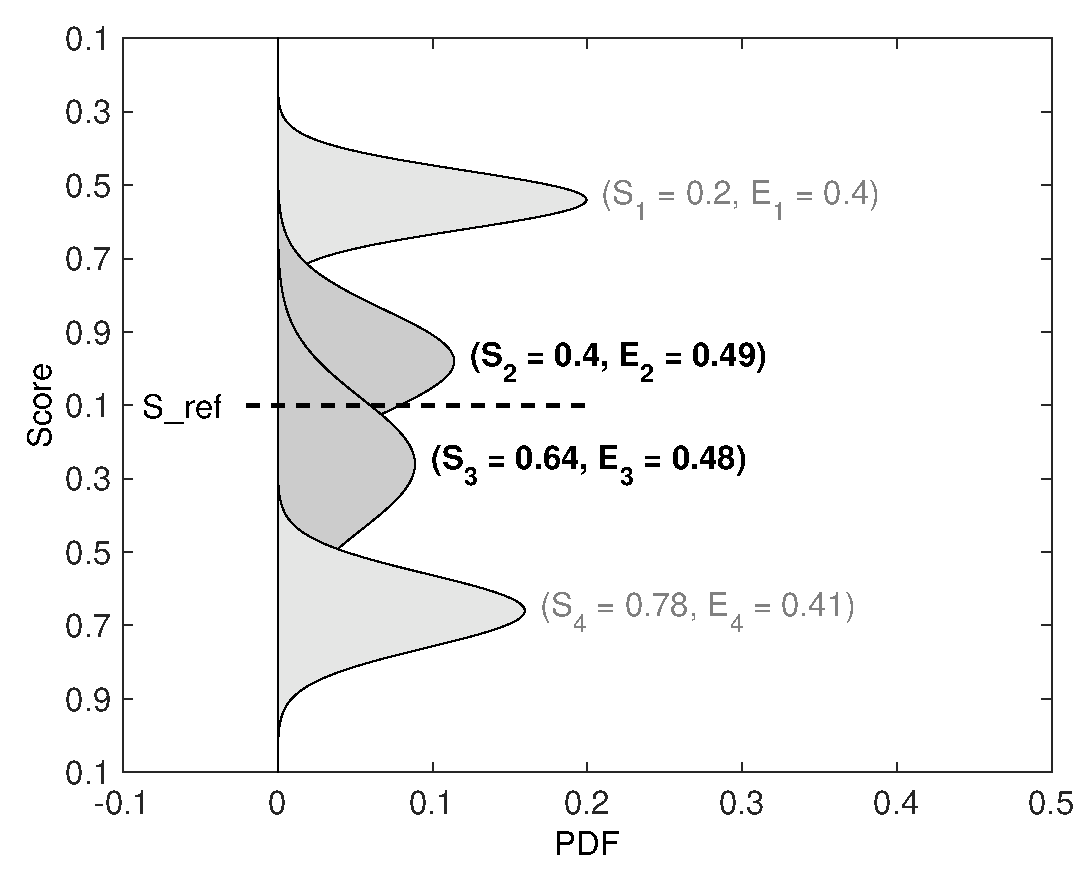
\includegraphics[scale=.28]{Figures/evaluation_principle.eps}
	\caption{Evaluation principle}
	\label{fig:evaluation_principle}
\end{figure}

\noindent\textbf{Reduce}: The above two stages: \textbf{Rank} and \textbf{GetSolutionEval} are repeated through all the fidelity levels of all objectives and/or all constraints till no solutions are selected for evaluation. In any generation, if $n\_HF$ = $0$, the solutions which do not have evaluated values of highest fidelity function in either of objective(s) and/or all constraints are identified. The top solution from this set is evaluated in the highest fidelity level of objective(s) and/or all constraints and added to the appropriate archives outlined in Steps 28--38 of Algorithm \ref{alg:MFEA}. Following this process, the combined population of parent and child solutions goes through the \textbf{Rank} process and the top $N$ solutions are carried forward as parents for the next generation.

\section{Performance Metrics}
For all the problems studied in the paper, we assume that for each problem, one has a limited computational budget prescribed by the user. The performance of the approach for single objective optimization is based on the quality of final solutions delivered and the rate of convergence. As for the multi-objective optimization problems, this merit is based on hypervolume metric defined  using Equation \ref{eq:hv}.

\begin{equation}\footnotesize
\text{HYP}(r) := \text{VOL}\left(\underset{f\_i,\forall i = 1,\ldots,r} \cup \left[f^{N}_1,f\_i_{1}\right]\times\ldots\left[f^{N}_{M},f\_i_{M}\right]\right)
\label{eq:hv}
\end{equation}
where $f\_i$ ($i = 1,\dots,r$) denotes the $M$ objective values of $i^{th}$ solution in the nondominated set of solutions of size $r$ and $\textbf{f}^{N}$ denotes the Reference point (usually nadir point). 

To compute the HV value at a given computational cost, all nondominated solutions evaluated so far are considered.  For HV computation, there are recent reports that suggest use of a slightly larger than true nadir point as a reference point \cite{auger2009theory,Yuan2016many,ishibuchi2010many}. In the context of multi-objective optimization problems, where the theoretical Pareto front is unknown, the archives (based on the highest fidelity values) across all independent optimization runs using all approaches are combined. The nadir point of the nondominated solutions obtained from this combined set is used to construct the reference point (i.e. reference point = $1.1\times$nadir point). Otherwise, the reference point is considered as 1.1 times the theoretical nadir point. The ideal point is also computed based on the nondominated solutions from the combined set. For any optimization run, at a given computational cost, all nondominated solutions evaluated (based on highest fidelity level) so far are considered. Given this set of nondominated solutions and their corresponding objective vectors, we first discard all solutions that lie outside the hyperbox formed between ideal and nadir points. The objective vectors of the remaining solutions are normalized using the ideal and the nadir vector listed under respective multi-objective problem description below and HV is computed using a reference point as $1.1^M$ ($M$ is the number of objectives for a given problem). All HV computations reported in this paper is based on the Monte Carlo simulation proposed in \cite{bader2011hype}.

\section{Numerical Results}\label{sec:results}
First, we illustrate the performance of the proposed approach on unconstrained optimization problems i.e. a single variable, single objective test problem and an eight variable single objective unconstrained optimization problem involving design of an underwater vehicle for minimum drag. For the underwater vehicle design problem, objective functions in various fidelity levels are based on Kriging models built from data obtained from computational fluid dynamics (CFD) simulations at various iterations. The performance of the proposed approach is then presented on two unconstrained multi-objective optimization problems i.e. a two variable, unconstrained multi-objective test problem and a three variable problem related to kinematics of flapping wings. Once again for the flapping wing problem, the objective functions in various levels of fidelity are based on Kriging models built from data obtained from computational fluid dynamics (CFD) simulations at various iterations. Thereafter, the performance of the algorithm is presented on two (one single objective and one multi-objective) constrained optimization problems.

For the mathematical test functions, results are based on 101 independent runs, while for the practical examples i.e. underwater vehicle and flapping wing kinematics, the results are based on 31 independent runs.The results of the proposed approach (PD-MFEA) is compared with results obtained using different single fidelity approaches and progressive fidelity approach. Since for a unknown problem, one would not be aware of the best fidelity level  to use, we present the results of an ``Average'' approach, which is equivalent to the average of the expected performances of different single fidelity approaches \cite{branke2016par}. For all the problems, the number of neighbors $n\_nb$ is set to four times the number of variables of the problem. The population size is set to ten times the number of variables of the problem. The probability of crossover is set to $1$ and a mutation probability of $0.1$ is used for all the problems, except for the toy submarine design and flapping wing design problems, wherein the mutation probability is considered as 1/$n$ (where $n$ is the number of variables of these problems). The distribution indices of crossover ($\eta_c$) and mutation($\eta_m$) are set to $20$ and $30$ respectively for all the problems considered in  this study. The convergence plot for an approach represents the median objective values (for single objective optimization problems) or HV values (for multi-objective optimization problems) obtained at specific cost. The number of function evaluations at different fidelity levels is presented for the optimization run of PD-MFEA corresponding to the median value of objective/HV obtained at the end of the computational budget.  

\subsection{Single objective unconstrained problems}

\subsubsection{Test function-I}
We illustrate the performance of the proposed strategy (PD-MFEA) using a single variable, single objective unconstrained minimization problem. The test function is presented in Figure \ref{fig:test_fn2mod} and the formulation is outlined in Equation \ref{eq:testfunc1}. There are $6$ fidelity levels for the function, where fidelity-1 ($SF^1$) is the least accurate costing $5$ units, fidelity-2 ($SF^2$) costs 10 units, fidelity-3 ($SF^3$) costs 15 units, fidelity-4 ($SF^4$) costs 20 units, fidelity-5 ($SF^5$) costs 25 units, and fidelity-6 ($SF^6$) corresponds to the most accurate estimate costing $75$ units of computational time. The properties of the test function at various levels of fidelity are listed in Table \ref{table:mse_tau_test_fn2mod}. The rank correlation coefficient and the mean squared error between the functions at various levels of fidelity are computed using $10,000$ uniformly spaced points. The theoretical optimum is located at $x$ = $-2$ and the fidelity-6 value corresponding to the optimum is $-32$.

\begin{figure}[!ht]
	\centering
	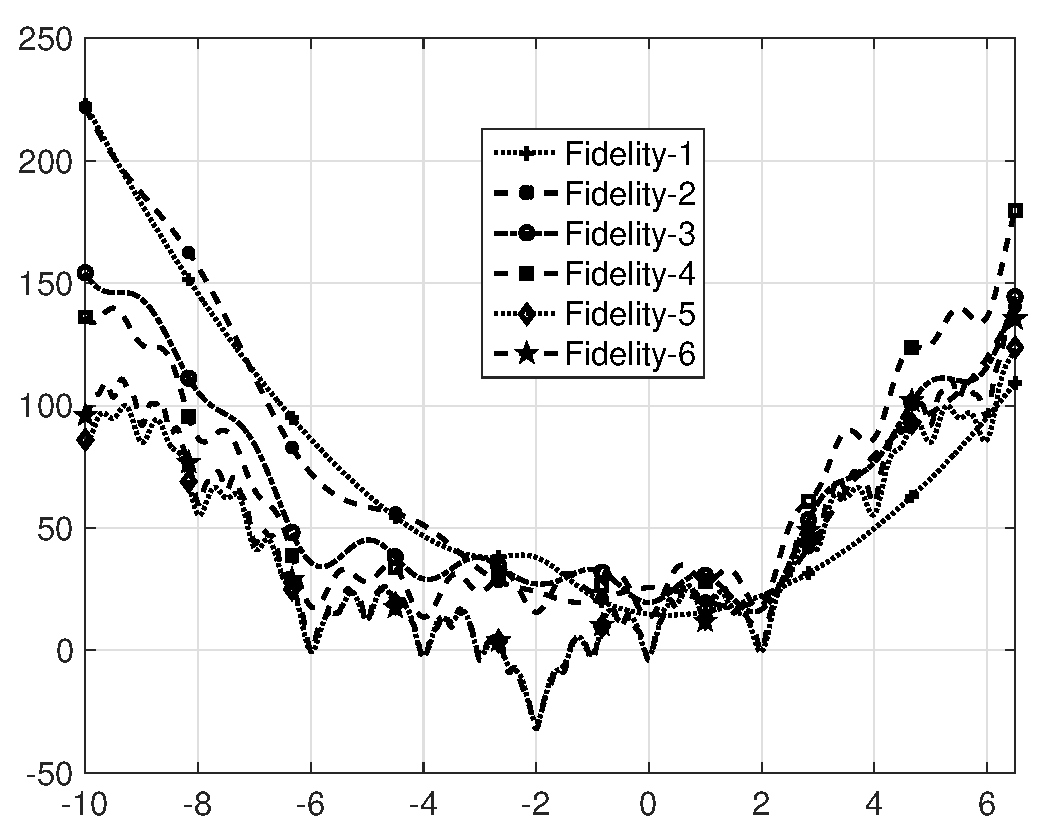
\includegraphics[scale=.28]{Figures/test_fn2mod.eps}
	\caption{Test function-I}
	\label{fig:test_fn2mod}       
\end{figure}

\begin{table}[!htb]\footnotesize
	\centering
	\caption{Test function-I: Mean squared error (MSE) and the rank correlation coefficient (Kendall Tau ($\uptau$)) between the fidelity levels}
	\label{table:mse_tau_test_fn2mod}
	\begin{tabular}{|c|c|c|c|c|c|c|}
		\noalign{\smallskip}\hline
		&$SF^1$&$SF^2$&$SF^3$&$SF^4$&$SF^5$&$SF^6$\\ \hline
		\textbf{MSE}&2235.467&2015.907&633.076&490.572&32.766&0.000\\ \hline
		\textbf{$\uptau$}&0.452&0.582&0.675& 0.828& 0.959& 1.000\\ \hline
	\end{tabular}
\end{table}

To solve this problem, one can opt to use any single fidelity approaches within an optimization scheme and evaluate the final population using the highest fidelity function. As an example, the cost of running an optimization exercise using fidelity-1 ($SF^1$) estimate for $3$ generations would be $900$ units. The cost breakdown is as follows: $50$ cost units to evaluate the initial population of $10$ individuals at generation $0$, $50$ units each for child solutions created in generations $1$, $2$ and $3$ i.e a total of $150$ units and the cost of evaluating the parent population at the end of generation $3$ to the highest level of fidelity i.e. $SF^6$ costing $700$ units. Take note that at the end of generation 3, all parent solutions have already have been evaluated in fidelity-1 and an evaluation in fidelity-6 would require an additional cost of $700$ units ($(75-5)\times 10$). The best solution for an evaluation budget of $900$ units would correspond to the best solution of the population at generation $3$, evaluated using $SF^6$. A population size of $10$ is used with the total evaluation budget limited to $10,000$ units to solve this problem. The performance of PD-MFEA is compared with other single fidelity approaches and progressive fidelity approach based on the results obtained from 101 runs and presented in Table \ref{tab:test_fn2mod_all}. 

\begin{table}[!htb]\footnotesize
	\caption{Test function-I: Final objective values of multi-fidelity, single fidelity optimization and progressive fidelity optimization}
	\label{tab:test_fn2mod_all}
	\centering
	\begin{tabular}{|c|c|c|c|c|c|}
		\noalign{\smallskip}\hline
		Approaches& Best &Mean & Median & Worst & Std Error\\ \hline
		$MF$&-31.999&-31.295&-31.992&-4.010&0.368\\ \hline
		$SF^1$&19.279&19.349&19.348&19.412&0.002\\ \hline
		$SF^2$&2.967&15.103&15.335&16.368&0.173\\ \hline
		$SF^3$&9.141&9.529&9.538&9.862&0.011\\ \hline
		$SF^4$&-4.015&-3.947&-3.958&-3.714&0.005\\ \hline
		$SF^5$&-31.999&-31.995&\textbf{-31.998}&-31.957&0.000\\ \hline
		$SF^6$&-31.999&-31.373&-31.917&-11.833&0.219\\ \hline
		$PF$&-31.997&-7.768&-0.057&0.635&1.159\\ 
		\hline
	\end{tabular}
\end{table}          

Apart from single fidelity approaches, one can also opt to use progressive fidelity models, wherein analysis models are progressively switched from lower fidelity level to higher fidelity levels over the course of evolution. In our progressive fidelity model, we assume that each fidelity model is used for $1/6^{th}$ of the computational budget.

The results of multi-fidelity, single fidelity and progressive fidelity optimization approaches corresponding to $s_{th}$ = 1  are presented in Table \ref{tab:test_fn2mod_all}. The example clearly illustrates that the use of lower fidelity models i.e $SF^1$ through to $SF^4$ and progressive fidelity approach would misguide the search. Based on the median values, use of $SF^5$ offers the best performance followed by multi-fidelity approach (PD-MFEA). 

\begin{figure}[ht]
	\centering
	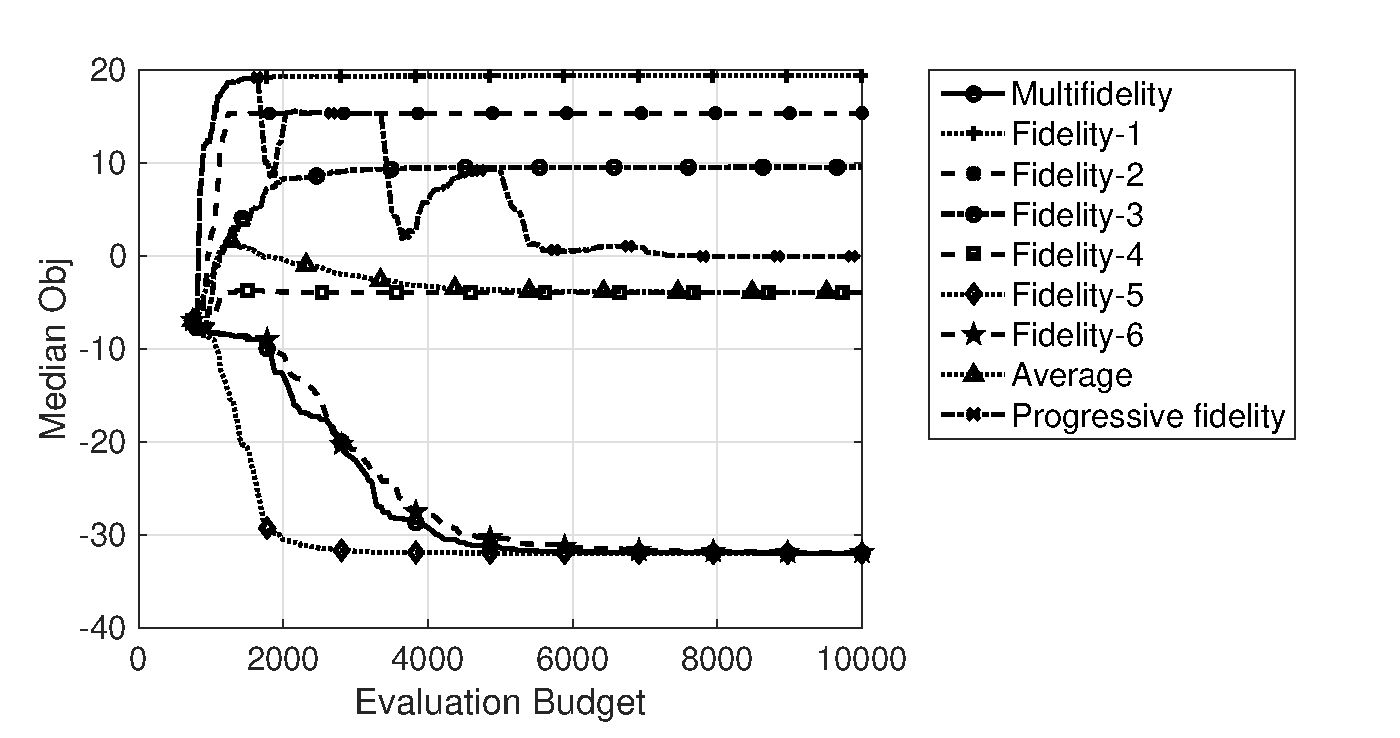
\includegraphics[scale=.35]{Figures/test_fn2mod_f.eps}
	\caption{Test function-I: Convergence with $s_{th}$ = 1}
	\label{fig:Meanplot_test_fn2mod_1sigma}
\end{figure}

\begin{figure}[ht]
	\centering
	\subfigure[]{\label{fig:Meanplot_test_fn2mod_k1k2}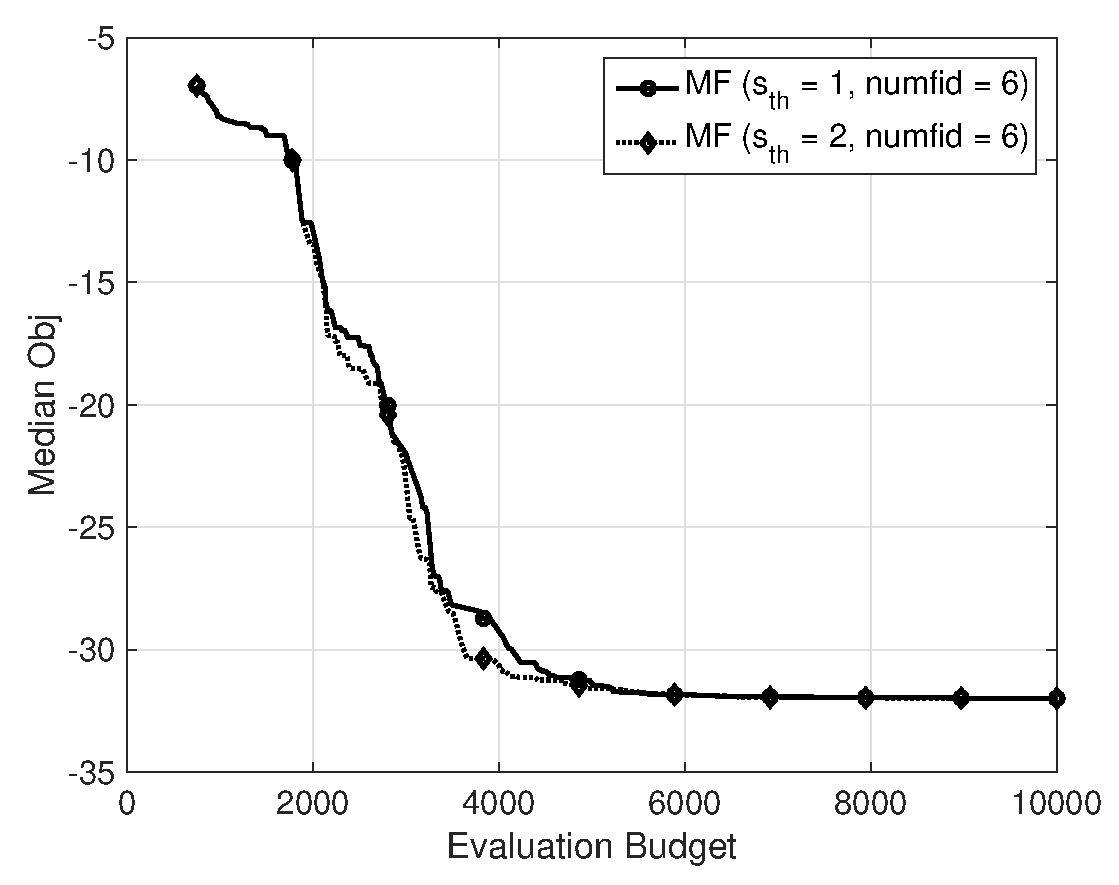
\includegraphics[scale=.27]{Figures/test_fn2modk1k2.eps}}
	\subfigure[]{\label{fig:Meanplot_test_fn2mod_k12}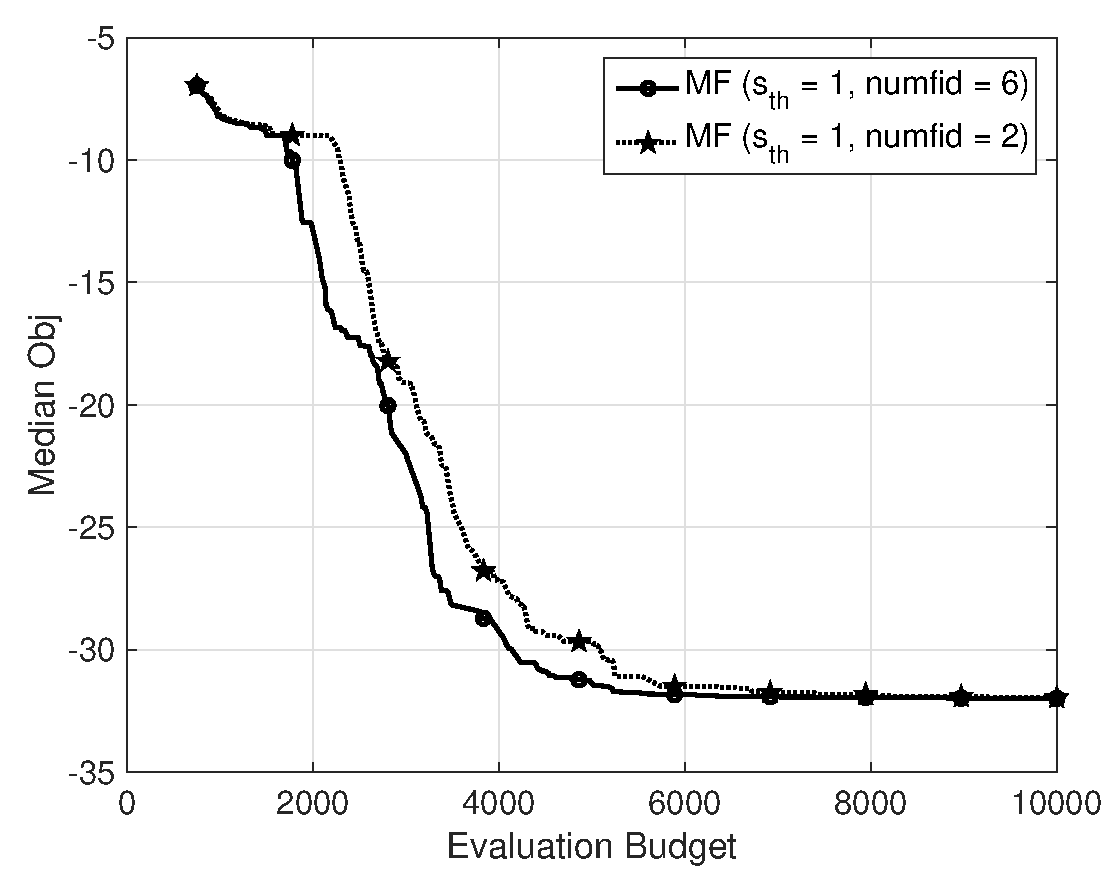
\includegraphics[scale=.27]{Figures/test_fn2modk12.eps}}
	\caption{Test function-I: (a) Convergence comparison of multi-fidelity approaches with $s_{th}$ = 1 and 2, (b) Convergence comparison of multi-fidelity approaches based on 6 fidelity levels and 2 fidelity levels with $s_{th}$ = 1}
	\label{fig:convergence_numfideval_test_fn2mod}
\end{figure}

The median convergence plots obtained using the multi-fidelity (corresponding to $s_{th}$ = 1), various single fidelity, and progressive fidelity approaches along with the average performance are shown in Figure \ref{fig:Meanplot_test_fn2mod_1sigma}. It can be easily observed that, $SF^5$ performs best followed by multi-fidelity approach and it works better than the highest fidelity and the average approaches. Therefore, in the absence of any prior information of the best approach, multi-fidelity approach is most reliable for this problem. 

In this problem, we had six levels of fidelity and assumed $s_{th}$ of 1. We investigate the effects of both i.e. a scenario where there are only two levels of fidelity i.e. $SF^1$ and $SF^6$ with a cost of $5$ and $75$ units, and the effect of choosing $s_{th}$ of 1 instead of 2.  Clearly $s_{th}$ of 2 is a more conservative setting than $s_{th}$ of 1 and more solutions are likely to be evaluated in every generation. A value of $s_{th}$ of 2 would also mean the underlying models will have a greater opportunity to get better.  In terms of the number of fidelity levels, we  expect that having six levels of fidelity offer an opportunity to exploit low fidelity estimates if they are well correlated with the highest fidelity function. Results presented in Figure \ref{fig:convergence_numfideval_test_fn2mod} clearly support the above hypothesis. One can observe that with $s_{th}$ of 2, more solutions get evaluated in higher levels of fidelity which in turn improves the approximation and offers better convergence. Furthermore, multi-fidelity optimization involving six fidelity levels perform better than multi-fidelity optimization with two levels of fidelity in most stages of evolution.

The following Figure \ref{fig:test_fn2mod_Numfideval_obj1_1sigma} presents the function evaluation in various fidelity levels for multi-fidelity approach corresponding to the optimization run delivering median final performance.  

\begin{figure}[ht]
	\centering
	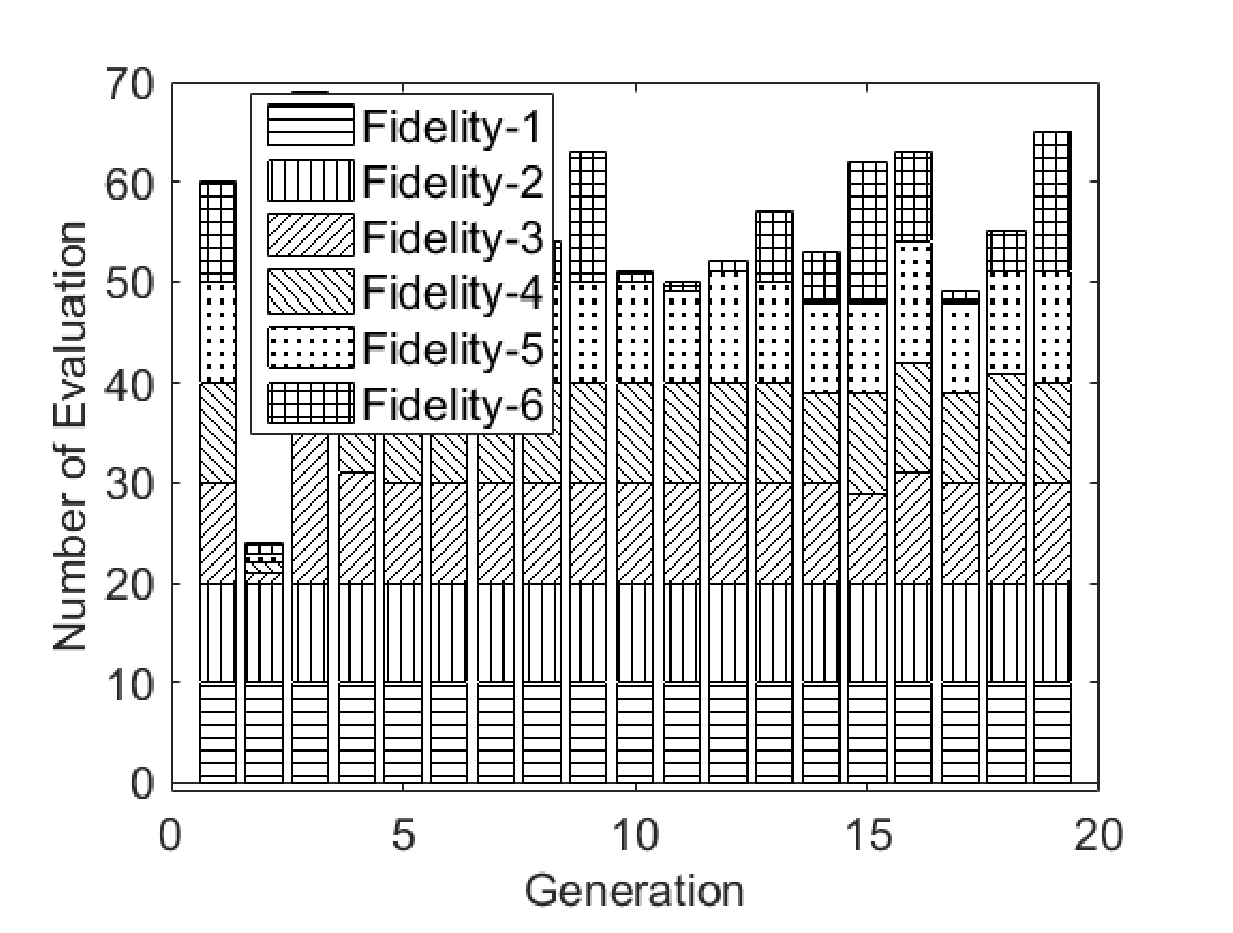
\includegraphics[scale=.28]{Figures/test_fn2mod_numeval.eps}
	\caption{Test function-I:Number of evaluations in various fidelity levels at $s_{th}$ = 1}
	\label{fig:test_fn2mod_Numfideval_obj1_1sigma}
\end{figure}

The following subsection shows the performance of the proposed strategy (PD-MFEA) on a practical problem (a eight variable single-objective unconstrained underwater vehicle design problem henceforth referred as ``Toysub'').

\subsubsection{Toysub}
The variables defining the geometry of the underwater vehicle are illustrated in Figure \ref{fig:dallas_photo}. The objective is to minimize drag. The design variables are: the position of the internal components along the $Z$-axis i.e. the position of the controller ($Z_C$), position of the propeller unit for pitch ($Z_V$) and yaw ($Z_L$) movements, position of the battery compartment ($Z_B$), smaller diameter ($d_t$) and length ($l_t$) of the tail and shape variation coefficient ($n_n$) and length ($l_n$) of the nose. The bounds of the variables are presented in Equation \ref{eq:formulation_toysub}.

For this problem, 396 designs were generated using Latin Hypercube Sampling (based on ``maximin'' criterion) and their drag was estimated using ANSYS FLUENT 13.0. Since the body is axisymmetric, a quarter model of the bare hull was used to reduce the CFD analysis costs. The velocity at the inlet was set to $0.5$ m/s, while that at the outlet was set to zero. 

\begin{figure}[!htb]
	\centering
	\includegraphics[width=2.6 in]{Figures/Dallas_Photo.eps}
	\caption{USS Dallas RC toy submarine}
	\label{fig:dallas_photo}       
\end{figure}

\begin{figure}[!ht]
	\centering
	\includegraphics[width=2.6in]{Figures/Design_Variables.pdf}
	\caption{Design variables}
	\label{fig:toysub_param_illum}      
\end{figure}

\begin{equation}\footnotesize
\begin{array}[p]{l}
\text{Minimize:}f\left(1\right) = D \\
\text{Variable bounds:}
\\
0 \le Z_C \le 300~mm;~~0 \le Z_V \le 300~mm
\\
0 \le Z_B \le 300~mm;~~0 \le Z_L \le 300~mm
\\
35 \le d_t \le 50~mm;~~80 \le l_t \le 150~mm
\\
1.5 \le n_n \le 3;~~45 \le l_n \le 100~mm
\label{eq:formulation_toysub}
\end{array}
\end{equation}

The drag values obtained after $5$, $10$, $25$, $50$, $75$ and $100$ iterations (cost units) were captured for all the $396$ designs. From this data,  six Gaussian Process models were built reflecting different fidelity levels. The mean squared error and the rank correlation coefficient (Kendall Tau) between the various fidelity estimates are presented below based on 10,000 Latin Hypercube Sampling presented in Table \ref{table:mse_tau_toysub}.

\begin{table}[!htb]\footnotesize
	\centering
	\caption{Toysub: Mean squared error (MSE) and the rank correlation coefficient (Kendall Tau ($\uptau$)) between the fidelity levels}
	\label{table:mse_tau_toysub}
	\begin{tabular}{|c|c|c|c|c|c|c|}
		\noalign{\smallskip}\hline
		&$SF^1$&$SF^2$&$SF^3$&$SF^4$&$SF^5$&$SF^6$\\ \hline
		\textbf{MSE}&1.608E-02&1.128E-03&1.919E-03&8.895E-05&2.273E-05&0.000\\ \hline
		\textbf{$\uptau$}&0.637&0.699&0.761& 0.869& 0.880& 1.000\\ \hline
	\end{tabular}
\end{table}

A population size of $80$ was used with a total computational budget of $100,000$ cost units. In this single-objective example, the performance of PD-MFEA is compared with all single fidelity, average and progressive fidelity approaches based on $31$ independent runs.

\begin{table}[!htb]\footnotesize
	\caption{Toysub: Final objective values of multi-fidelity, single fidelity optimization and progressive fidelity optimization}
	\label{tab:toysub_all}
	\centering
	\begin{tabular}{|c|c|c|c|c|c|}
		\noalign{\smallskip}\hline
		Approaches& Best &Mean & Median & Worst & Std Error\\ \hline
		$MF$&0.075&0.077&\textbf{0.076}&0.081&0.000\\ \hline
		$SF^1$&0.079&0.103&0.100&0.121&0.003\\ \hline
		$SF^2$&0.076&0.078&0.077&0.086&0.000\\ \hline
		$SF^3$&0.077&0.078&0.077&0.084&0.000\\ \hline
		$SF^4$&0.075&0.077&\textbf{0.076}&0.083&0.000\\ \hline
		$SF^5$&0.076&0.077&\textbf{0.076}&0.083&0.000\\ \hline
		$SF^6$&0.076&0.078&0.077&0.083&0.000\\ \hline
		$PF$&0.076&0.083&0.083&0.092&0.000\\ 
		\hline
	\end{tabular}
\end{table}

The results of multi-fidelity ($s_{th}$ = 1 ), single fidelity and progressive fidelity approaches are presented in Table \ref{tab:toysub_all}. Based on median final objective values, multi-fidelity approach (PD-MFEA), $SF^4$ and $SF^5$ offer the best performance. 

The median convergence plot obtained using the multi-fidelity approach (corresponding to $s_{th}$ = 1), various single fidelity approaches, and progressive fidelity approach along with the average performance are shown in Figure \ref{fig:Meanplot_toysub_1sigma}. One can observe that (a) use of lowest fidelity and progressive fidelity scheme would misguide the search completely, (b) use of fidelity 2, 3 and 4 will offer higher convergence during the initial stages due to lower cost of evaluation and finally (c) the use of highest fidelity approach is not attractive as it demands significant computational cost.

\begin{figure}[ht]
	\centering
	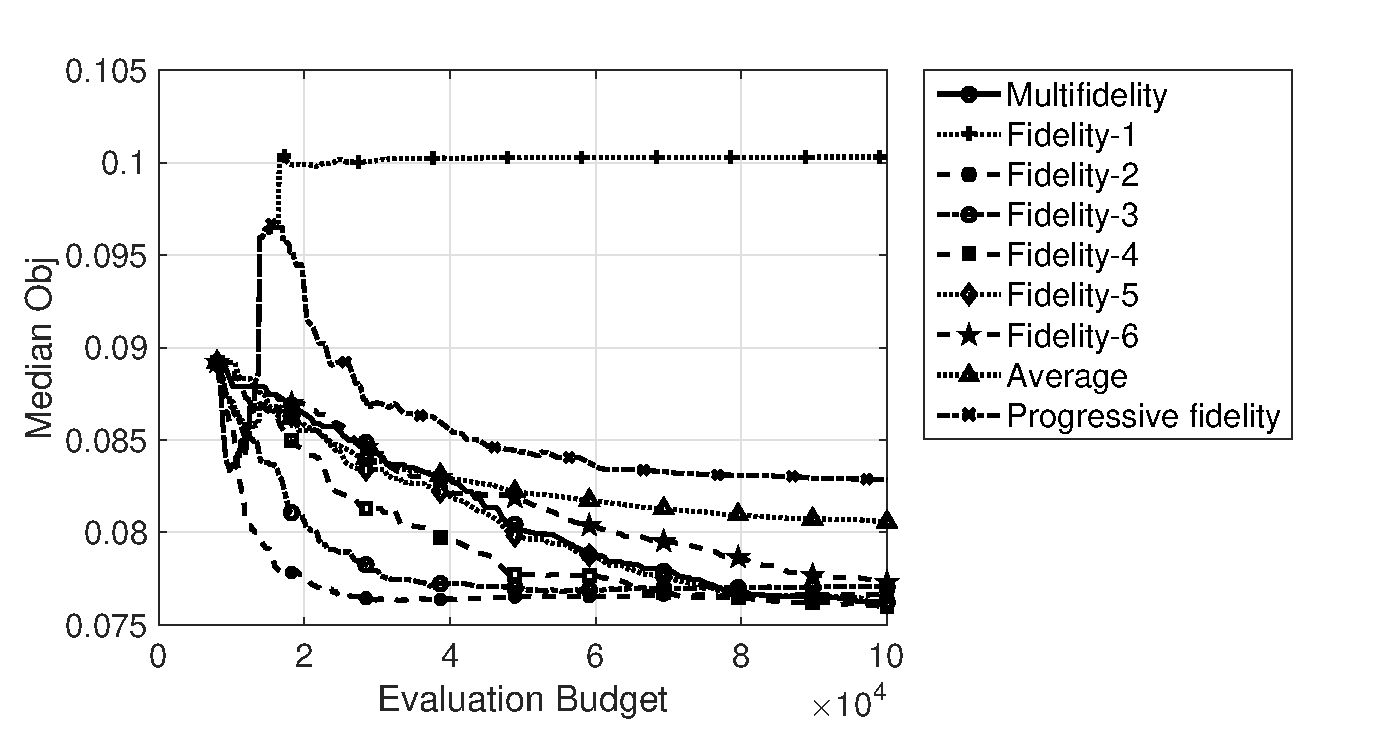
\includegraphics[scale=.35]{Figures/toysub_f.eps}
	\caption{Toysub: Convergence with $s_{th}$ = 1}
	\label{fig:Meanplot_toysub_1sigma}
\end{figure}

\subsection{Multi-objective unconstrained problems}
In this section we present the performance of the proposed approach using two unconstrained multi-objective optimization problems i.e. a mathematical test problem and a practical problem involving design of flapping wing kinematics. 
\subsubsection{Test function-II}

This test function consists of two objectives ($f_1$ and $f_2$, that need to be minimized) defined using three variables ($x_i$, for $i = 1,2,3$). There are $6$ fidelity levels for this function in each objective, where fidelity-1 ($SF^1$) is the most inaccurate costing $5$ units, fidelity-2 ($SF^2$) costs 10 units, fidelity-3 ($SF^3$) costs 15 units, fidelity-4 ($SF^4$) costs 20 units, fidelity-5 ($SF^5$) costs 50 units, and fidelity-6 ($SF^6$) corresponds to the most accurate estimate costing $100$ units of computational time. 

In this example, we have shown the theoretical Pareto fronts in the lowest and highest fidelity in Figure \ref{fig:fspaceparetoalltestfunc2} using $10,000$ solutions obtained from Latin Hypercube sampling. The formulation of the first objective is shown in Equation \ref{eq:testfunc2}, while for the second objective, all $\sin$ functions are replaced by $\cos$ functions. 

\begin{figure}[ht]
	\centering
	\includegraphics[scale = 0.40]{Figures/NDobj_Fidelity.eps}
	\caption{Theoretical Pareto fronts of Test function-II}
	\label{fig:fspaceparetoalltestfunc2}
\end{figure}

The following values in Table \ref{tab:testfunc2loc} are of the variables $x_2$ and $x_3$ which correspond to global optima of different fidelity levels.

\begin{table}[!htb]\footnotesize
	\caption{Test function-II: Location of optimum in $2^{nd}$ and $3^{rd}$ variables}
	\label{tab:testfunc2loc}
	\centering
	\begin{tabular}{|c|c|c|c|c|c|c|}
		\noalign{\smallskip}\hline
		&$SF^1$&$SF^2$&$SF^3$&$SF^4$&$SF^5$&$SF^6$\\ \hline
		$x_2$&0.600&0.500&0.400&0.300&0.240&0.200\\ \hline
		$x_3$&0.500&0.600&0.700&0.820&0.860&0.900\\ \hline
	\end{tabular}
\end{table}

The mean squared error and the rank correlation coefficient (Kendall Tau) among various fidelity levels based on $10,000$ latin hypercube sampled random designs are listed in Table \ref{tab:mse_tau_testfunc2}.

\begin{table}[!htb]\footnotesize
	\centering
	\caption{Test function-II: Mean squared error (MSE) and the rank correlation coefficient (Kendall Tau ($\uptau$)) between the fidelity levels}
	\label{tab:mse_tau_testfunc2}
	\begin{tabular}{|l|l|l|l|l|}
		\noalign{\smallskip}\hline
		& \textbf{Objective-1} &                      & \textbf{Objective-2} &                      \\ \hline
		& \textbf{MSE}         & \textbf{$\uptau$} & \textbf{MSE}         & \textbf{$\uptau$} \\ \hline
		\textbf{$SF^1$} & 5.903E+04           & 0.236               & 5.799E+04           & 0.256               \\ \hline
		\textbf{$SF^2$} & 4.142E+04           & 0.428               & 4.134E+04           & 0.444               \\ \hline
		\textbf{$SF^3$} & 1.464E+04           & 0.582               & 1.486E+04           & 0.604               \\ \hline
		\textbf{$SF^4$} & 4.374E+03           & 0.758               & 4.413E+03           & 0.772               \\ \hline
		\textbf{$SF^5$} & 0.686E+03           & 0.936               & 0.706E+03           & 0.937               \\ \hline
		\textbf{$SF^6$} & 0.000E+00           & 1.000               & 0.000E+00           & 1.000               \\ \hline
	\end{tabular}
\end{table}

For this problem, it is challenging for any optimizer to reach the Pareto front. A population size of $30$ is used with a total evaluation budget limited to $50,000$ units. In this bi-objective example, the performance of PD-MFEA is compared with all single fidelity and progressive fidelity approach in terms of rate of convergence and final values of median hypervolume obtained from $101$ independent optimization runs. For this example, we have used [37,38] as the reference point and [0,0] as ideal point to compute the hypervolume values. The convergence plots with$s_{th}$ = 1 is presented in Figure \ref{fig:testfunc2_1sigma}. During initial stages of evolution, use of fidelity-5 shows significant benefit, however it is misguided after a while. The final HV statistics of all the approaches including multi-fidelity approaches for $s_{th}$ = 1 are presented in Table \ref{tab:testfunc2hvstat}. It is clear that multi-fidelity approach offers the best performance based on the median statistics. 

\begin{figure}[!ht]
	\centering
	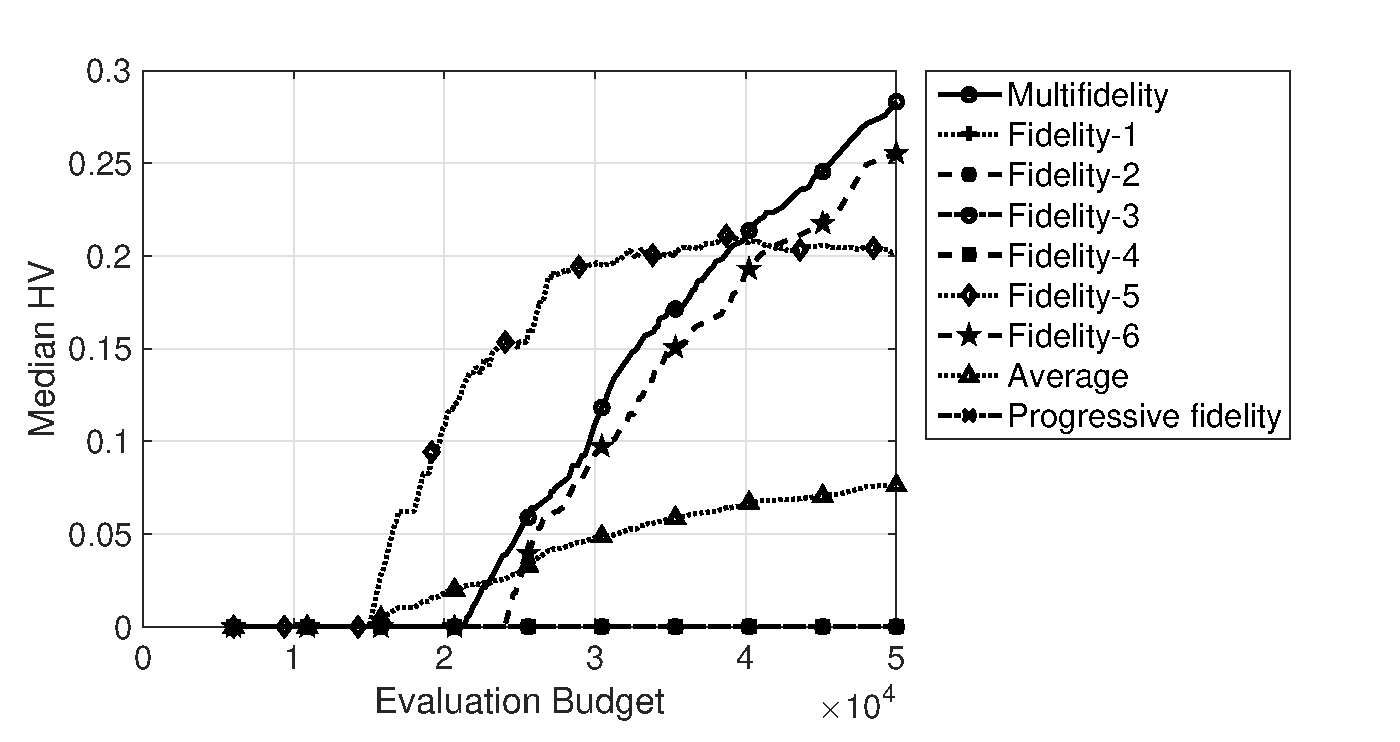
\includegraphics[scale=.35]{Figures/test_new_HV.eps}
	\caption{Test function-II: HV convergence with $s_{th}$ = 1}
	\label{fig:testfunc2_1sigma}
\end{figure}

We now move on to an interesting scenario when there are redundant fidelity levels, i.e. if fidelity-4,fidelity-5 and fidelity-6 have a rank correlation of 1.0. Ideally, we would expect the algorithm to detect this and avoid evaluation in fidelity-5 or fidelity-6. Results of number of evaluations performed in various fidelity levels for this problem is presented in Figure \ref{fig:testfunc2redundant}. They clearly indicate that PD-MFEA does not evaluate any solution in  fidelity-5 and fidelity-6 apart from during initialization.

\begin{figure}[!h]
	\centering
	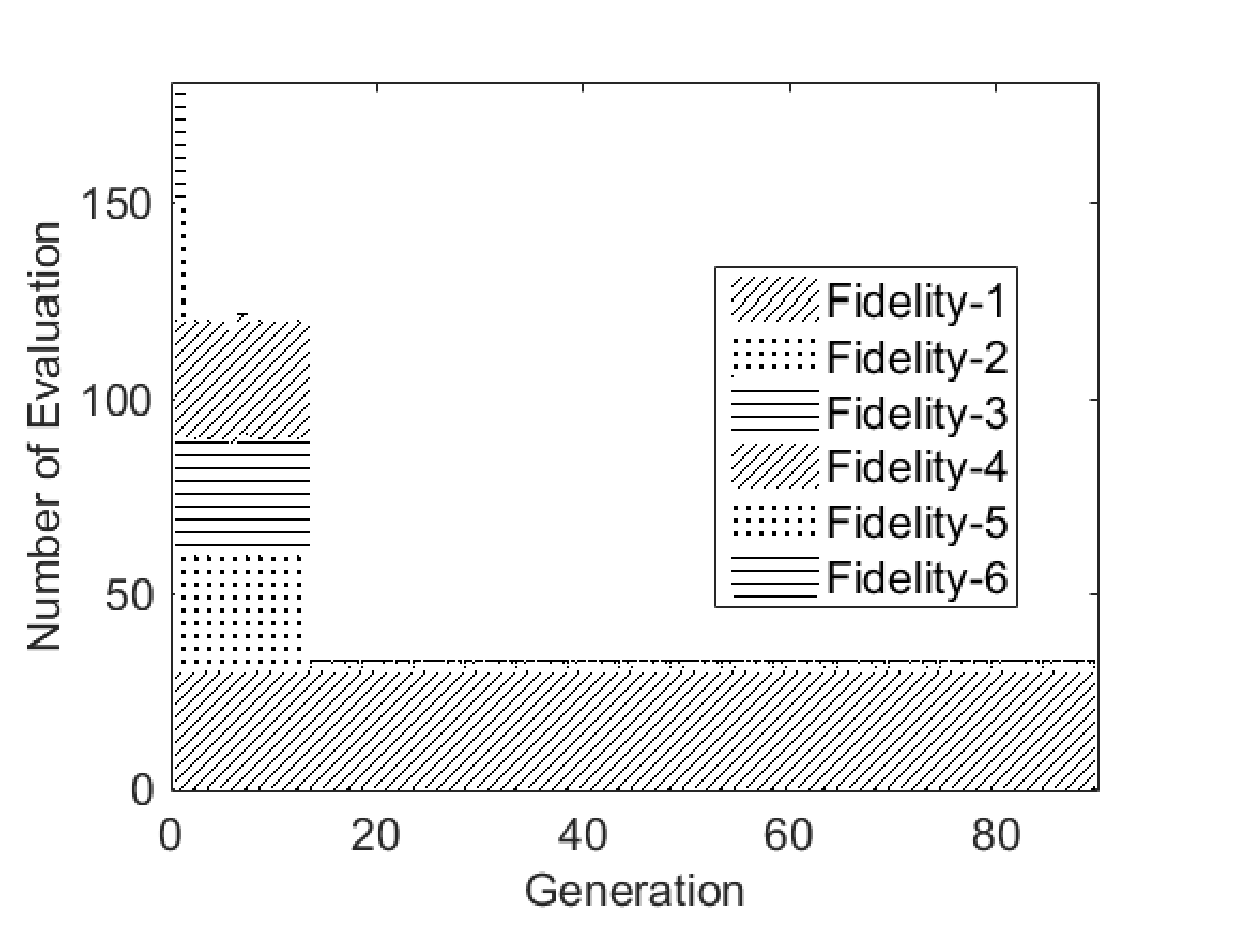
\includegraphics[scale=.31]{Figures/test_redundant_numeval.eps}
	\caption{Test function-II: Number of evaluations in various fidelity levels for redundant case}
	\label{fig:testfunc2redundant}      
\end{figure}

\begin{table}[!htb]\footnotesize
	\centering
	\caption{Test function-II: Final HV values of multi-fidelity, single fidelity optimization and progressive fidelity optimization}
	\label{tab:testfunc2hvstat}
	\begin{tabular}{|c|c|c|c|c|c|}
		\noalign{\smallskip}\hline
		Solver& Best &Mean & Median & Worst & Std Error\\ \hline
		$MF$&0.375&0.256&\textbf{0.283}&0.000&0.008\\ \hline
		$SF^1$&0.000&0.000&0.000&0.000&0.000\\ \hline
		$SF^2$&0.000&0.000&0.000&0.000&0.000\\ \hline
		$SF^3$&0.000&0.000&0.000&0.000&0.000\\ \hline
		$SF^4$&0.000&0.000&0.000&0.000&0.000\\ \hline
		$SF^5$&0.289&0.202&0.202&0.102&0.003\\ \hline
		$SF^6$&0.372&0.242&0.255&0.000&0.008\\ \hline
		$PF$&0.052&0.001&0.000&0.000&0.000\\ 
		\hline
	\end{tabular}
\end{table}

\subsubsection{Flapping wing}             

The performance of the proposed approach is also validated on a practical flapping wing kinematics problem involving three variables. The design variables are the reduced frequency ($x_1$), pivot point ($x_2$) and pitch amplitude ($x_3$). There are two objectives associated with this problem which needs to be maximized: power and efficiency. The range of the variables are $x_1~\in [0.6,1], x_2~\in [0.25,0.5]~\text{and}~x_3~\in [60,90]$. The power and efficiency values after $1$, $2$, $3$, $4$, and $5$ cycles (equivalent to $5$, $10$, $15$, $20$ and $50$ cost units) were captured for $111$ designs. From this data, five Kriging models were constructed representing analysis in each fidelity level. The mean squared error and the rank correlation coefficient (Kendall Tau) between the various fidelity estimates are presented below based on $10,000$ sampled points generated via LHS sampling. The properties of the functions at various levels of fidelity are listed in Table \ref{tab:mse_tau_flapping}.  

\begin{table}[!htb]\footnotesize
	\centering
	\caption{Flapping wing: Mean squared error (MSE) and the rank correlation coefficient (Kendall Tau ($\uptau$)) between the fidelity levels}
	\label{tab:mse_tau_flapping}
	\begin{tabular}{|l|l|l|l|l|}
		\noalign{\smallskip}\hline
		& \textbf{Objective-1} &                      & \textbf{Objective-2} &                      \\ \hline
		& \textbf{MSE}         & \textbf{$\uptau$} & \textbf{MSE}         & \textbf{$\uptau$} \\ \hline
		\textbf{$SF^1$} & 0.049           & 0.639               & 0.409           & 0.662               \\ \hline
		\textbf{$SF^2$} & 0.001           & 0.913              & 2.056E-04           & 0.868               \\ \hline
		\textbf{$SF^3$} & 3.192E-04           & 0.948               & 3.704E-05           & 0.941               \\ \hline
		\textbf{$SF^4$} & 1.992E-04           & 0.949               & 5.989E-06           & 0.971               \\ \hline
		\textbf{$SF^5$} & 0.000           & 1.000              & 0.000           & 1.000               \\ \hline
	\end{tabular}
\end{table}

A population size of $30$ was used with a total computational budget of $25,000$ units to solve this problem using PD-MFEA and compared with all the single fidelity approaches, progressive fidelity approach and average approach based on $31$ independent optimization runs.  

\begin{figure}[ht]
	\centering
	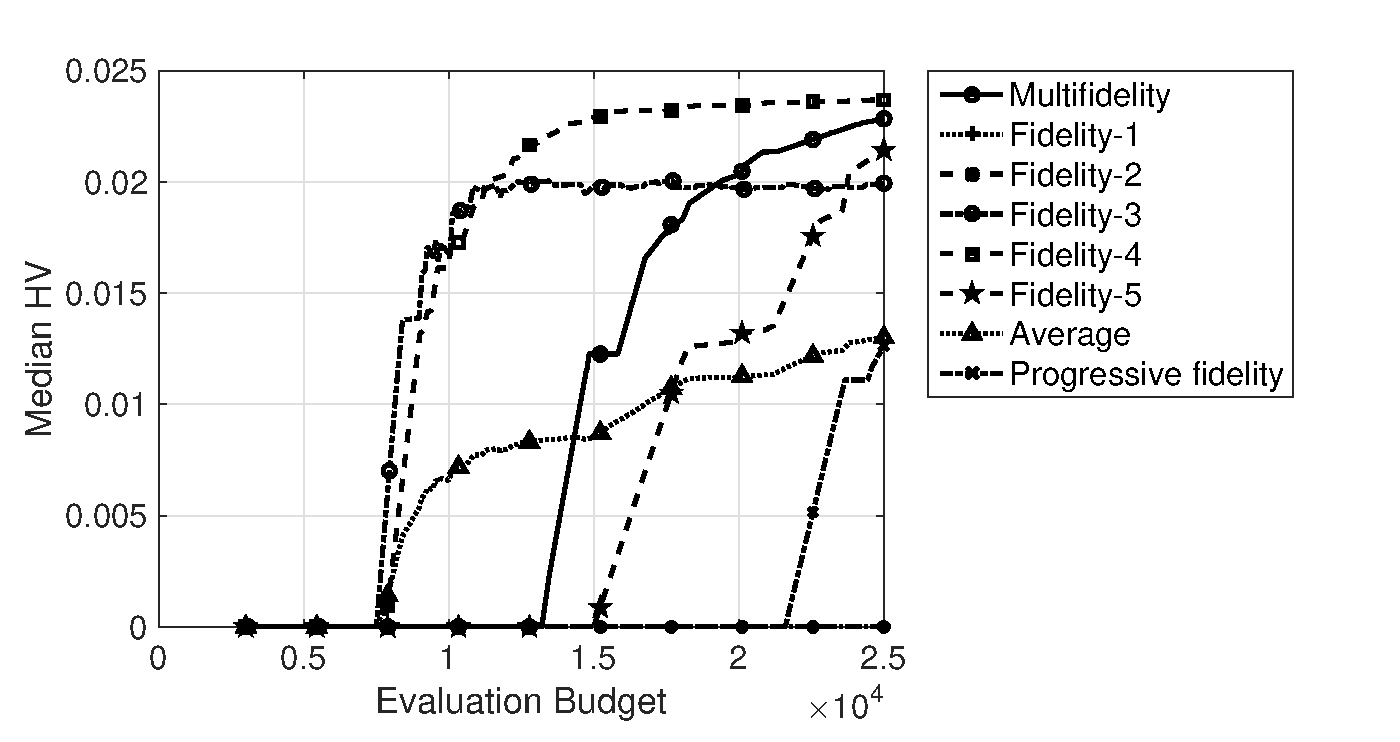
\includegraphics[scale=.35]{Figures/flapping_wing_HV.eps}
	\caption{Flapping wing: HV convergence at $s_{th}$ = 1}
	\label{fig:flapping_HV_1sigma}
\end{figure}

The median HV convergence plots of various strategies are compared with results obtained using PD-MFEA with a $s_{th}$ of 1. From Figure \ref{fig:flapping_HV_1sigma}, one can observe that the use of highest fidelity evaluation offers poor performance when compared to the multi-fidelity approach. The use of fidelity 3 and 4 offer better performance in general as they have high correlation with the highest fidelity level and is less expensive as can be observed from Figure \ref{fig:flapping_HV_1sigma}. For the computation of HV, we have collected results from all evaluated solutions from all runs. The reference point and the ideal point for this problem are considered as [-0.9411,-0.3519] and [-1,-0.5] respectively. 

The final statistics of the HV values corresponding to multi-fidelity optimization (corresponding to $s_{th}$ = 1), single fidelity approaches and progressive fidelity approach are presented in Table \ref{tab:flapping_HV}. According to Table \ref{tab:flapping_HV}, use of fidelity-4 offer the best performance followed by multi-fidelity approach in terms of median statistics. It is also clear that the use of highest fidelity approach and progressive fidelity approach are  poor choices.  

\begin{table}[!htb]\footnotesize
	\centering
	\caption{Flapping wing: Final HV values of multi-fidelity, single fidelity optimization and progressive fidelity optimization}
	\label{tab:flapping_HV}
	\begin{tabular}{|c|c|c|c|c|c|}
		\noalign{\smallskip}\hline
		Solver& Best &Mean & Median & Worst & Std Error\\ \hline
		$MF$&0.024&0.021&0.023&0.000&0.000\\ \hline
		$SF^1$&0.000&0.000&0.000&0.000&0.000\\ \hline
		$SF^2$&0.000&0.000&0.000&0.000&0.000\\ \hline
		$SF^3$&0.022&0.019&0.019&0.000&0.000\\ \hline
		$SF^4$&0.024&0.023&\textbf{0.024}&0.022&0.000\\ \hline
		$SF^5$&0.024&0.017&0.021&0.000&0.002\\ \hline
		$PF$&0.023&0.009&0.013&0.000&0.000\\ \hline
	\end{tabular}
\end{table}

\subsection{Single objective constrained problems}

\subsubsection{Test function-III}
In the previous sections we have illustrated the performance of PD-MFEA for unconstraned single and multi-objective optimization problems. Here we investigate its performance on two constrained optimization problems. The first is a single variable single objective constrained optimization problem. The constraint and the objective functions are illustrated in Figure \ref{fig:test_c1} and the formulation is presented in Equation \ref{eq:testfunc3}. There are $5$ fidelity levels associated with both the constraint and the objective functions, where fidelity-1 ($SF^1$) is the most inaccurate costing $5$ units, fidelity-2 ($SF^2$) costs 10 units, fidelity-3 ($SF^3$) costs 15 units, fidelity-4 ($SF^4$) costs 20 units, fidelity-5 ($SF^5$) corresponds to the most accurate estimate costing $50$ units of computational time. The properties of the test function at various levels of fidelity for both objective and constraint functions are listed in Table \ref{table:mse_tau_test_c1}. The rank correlation coefficient and the mean squared error between the functions at various levels of fidelity are computed using $10,000$ uniformly spaced points. The optimum is located at $x$ = $-3.375$ and the fidelity-5 value corresponding to this is $-0.146$. The feasible space for this problem lies within $x$ = 3.109 to 3.375 and it is around 5.20\% of the total search space.

\begin{figure}[!ht]
	\centering
	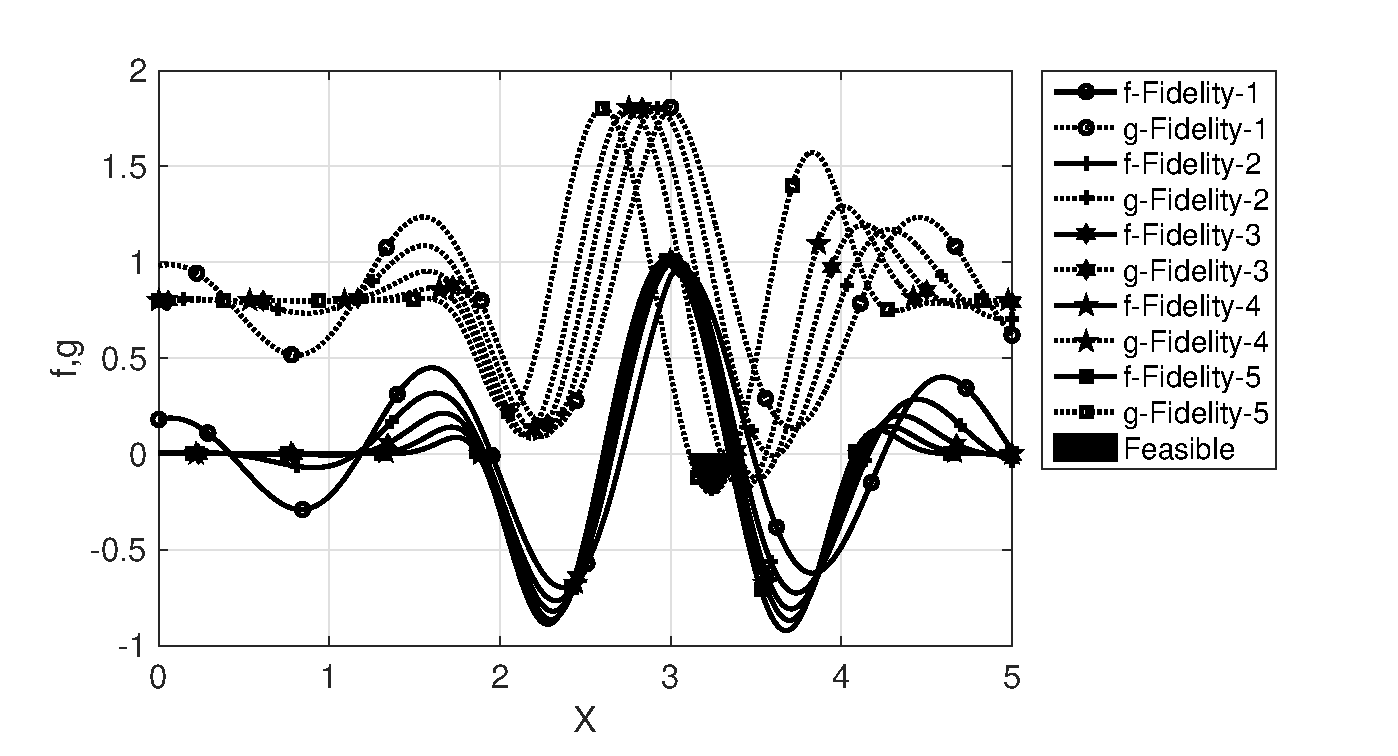
\includegraphics[scale=.35]{Figures/test_c1_fg.eps}
	\caption{Test function-III}
	\label{fig:test_c1}       
\end{figure}

\begin{table}[!htb]\footnotesize
	\centering
	\caption{Test function-III: Mean squared error (MSE) and the rank correlation coefficient (Kendall Tau ($\uptau$)) between the fidelity levels}
	\label{table:mse_tau_test_c1}
	\begin{tabular}{|l|l|l|l|l|l|}
		\noalign{\smallskip}\hline
		& \textbf{$SF^1$} & \textbf{$SF^2$} & \textbf{$SF^3$} & \textbf{$SF^4$} & \textbf{$SF^5$} \\ \hline
		\multicolumn{6}{|c|}{\textbf{Objective}}                                                                  \\ \hline
		\textbf{MSE}    & 0.080           & 0.024           & 0.008           & 0.002           & 0.000           \\ \hline
		\textbf{$\uptau$} & 0.601           & 0.774           & 0.871           & 0.927           & 1.000           \\ \hline
		\multicolumn{6}{|c|}{\textbf{Constraint}}                                                                 \\ \hline
		\textbf{MSE}    & 0.463           & 0.356           & 0.231           & 0.118           & 0.000           \\ \hline
		\textbf{$\uptau$} & -0.171          & 0.011           & 0.260           & 0.489           & 1.000           \\ \hline
	\end{tabular}
\end{table}


A population size of $10$ is used with the total evaluation budget limited to $20,000$ units to solve this problem. The performance of PD-MFEA is compared with other single fidelity approaches, progressive fidelity approach and average approach based on the results obtained from 101 independent optimization runs. 

\begin{figure}[ht]
	\centering
	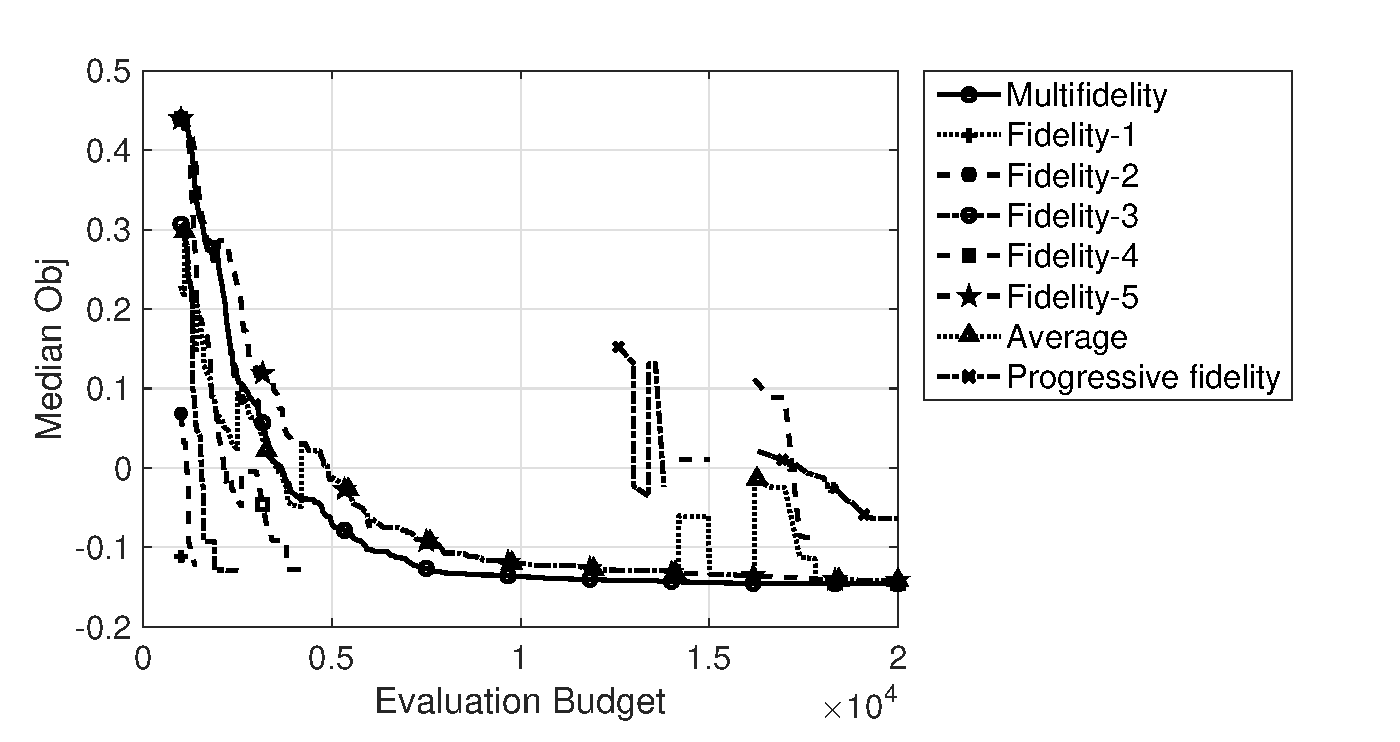
\includegraphics[scale=.35]{Figures/test_c1_f.eps}
	\caption{Test function-III: Convergence with $s_{th}$ = 1}
	\label{fig:Meanplot_test_c1_1sigma}
\end{figure}

The convergence of various strategies are presented in Figure \ref{fig:Meanplot_test_c1_1sigma}. It is clear that throughout the evolution, multi-fidelity approach works better than highest fidelity approach. In the context of average performance, it is same as performance obtained using highest fidelity approach except during the initial stages. All other single fidelity approaches except the use of highest fidelity evaluation failed to deliver feasible solutions in the end. 

\begin{figure}[ht]
	\centering
	\subfigure[]{\label{fig:test_c1_Numfideval_obj1_1sigma}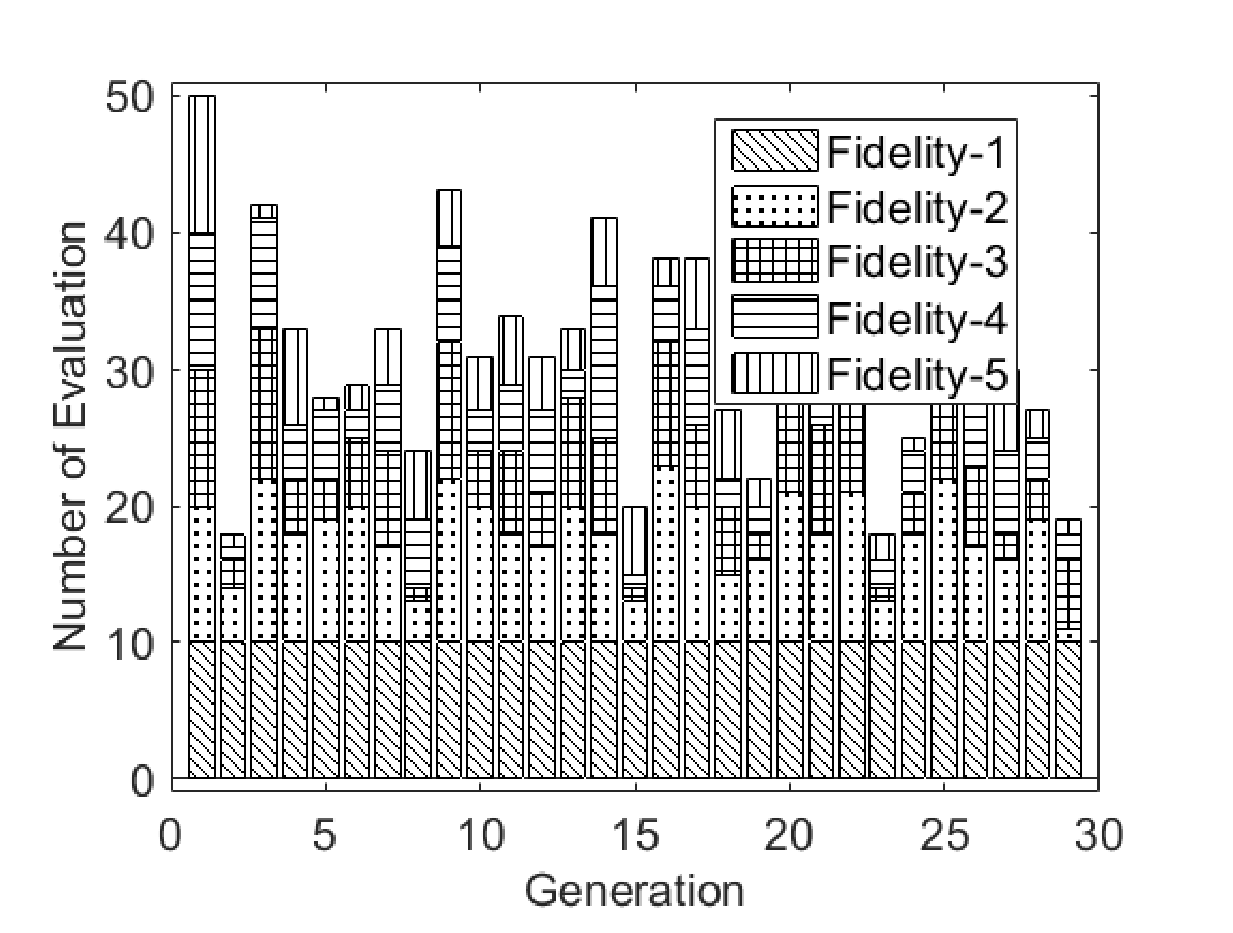
\includegraphics[scale=.30]{Figures/test_c1_numeval_f.eps}}
	\subfigure[]{\label{fig:test_c1_Numfideval_const1_1sigma}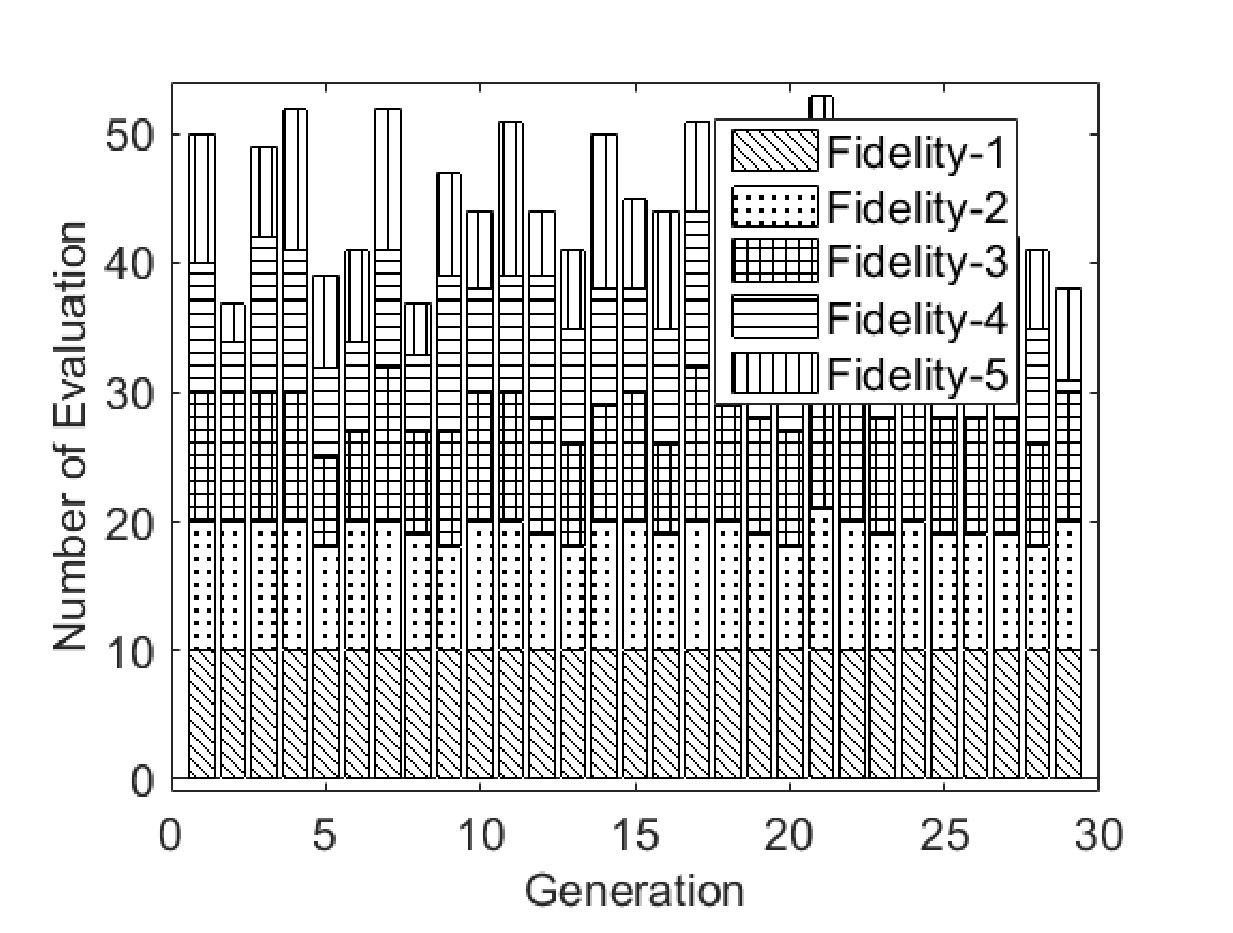
\includegraphics[scale=.30]{Figures/test_c1_numeval_g.eps}}
	\caption{Test function-III: Number of function evaluations in various fidelity levels at $s_{th}$ = 1 of (a) objective, (b) constraint}
	\label{fig:test_c1_evaluations}
\end{figure}

For this problem, one can notice poor correlation of the constraint function when compared to the objective functions in various fidelity levels. From Figure \ref{fig:test_c1_evaluations}, one can notice that there are larger number of higher fidelity evaluations for constraints than objectives which is a result of the above nature of the problem. Statistics at the end of evaluation budget for all runs corresponding to various approaches are listed in Table \ref{tab:test_c1_all}. Multi-fidelity approach outperforms highest fidelity and progressive fidelity approach throughout the course of evolution.  

\begin{table}[!htb]\footnotesize
	\caption{Test function-III: Final objective values of multi-fidelity, single fidelity optimization and progressive fidelity optimization}
	\label{tab:test_c1_all}
	\centering
	\begin{tabular}{|c|c|c|c|c|c|}
		\noalign{\smallskip}\hline
		Solver& Best &Mean & Median & Worst & Std Error\\ \hline
		$MF$&-0.147&-0.139&\textbf{-0.146}&0.244&0.004\\ \hline
		$SF^1$&NaN&NaN&NaN&NaN&NaN\\ \hline
		$SF^2$&NaN&NaN&NaN&NaN&NaN\\ \hline
		$SF^3$&NaN&NaN&NaN&NaN&NaN\\ \hline
		$SF^4$&NaN&NaN&NaN&NaN&NaN\\ \hline
		$SF^5$&-0.147&-0.135&-0.141&-0.056&0.001\\ \hline
		$PF$&-0.146&-0.033&-0.064&0.364&0.013\\ 
		\hline
	\end{tabular}
\end{table}


\subsection{Multi-objective constrained problem}

\subsubsection{Test function-IV}

To conclude, we present a constrained multi-objective test problem with the objective formulations same as test function-II. The formulation of the constraint function is outlined in Equation \ref{eq:testfunc4}. For this function, fidelity-1 ($SF^1$) is the most inaccurate costing $5$ units, fidelity-2 ($SF^2$) costs 10 units, fidelity-3 ($SF^3$) costs 15 units, fidelity-4 ($SF^4$) costs 20 units, fidelity-5 ($SF^5$) costs 50 units and fidelity-6 ($SF^6$) corresponds to the most accurate estimate costing $100$ units of computational time for both objective and constraint functions. The properties of the test function at various levels of fidelity are listed in Table \ref{table:mse_tau_test4}. The rank correlation coefficient and the mean squared error between the functions at various levels of fidelity are computed using $10,000$ uniformly spaced points. A population size of $30$ is used with the total evaluation budget limited to $100,000$ units to solve this problem.

\begin{table}[!htb]\footnotesize
	\centering
	\caption{Test function-IV: Mean squared error (MSE) and the rank correlation coefficient (Kendall Tau ($\uptau$)) between the fidelity levels}
	\label{table:mse_tau_test4}	
	\begin{tabular}{|l|l|l|l|l|l|l|}
		\noalign{\smallskip}\hline
		& \textbf{$SF^1$} & \textbf{$SF^2$} & \textbf{$SF^3$} & \textbf{$SF^4$} & \textbf{$SF^5$} & \textbf{$SF^6$} \\ \hline
		\multicolumn{7}{|c|}{\textbf{Objective-1}}                                                                                  \\ \hline
		\textbf{MSE}    & 5.903E+04       & 4.142E+04       & 1.464E+04       & 4.374E+03       & 0.686E+03       & 0.000E+00       \\ \hline
		\textbf{$\uptau$} & 0.236           & 0.428           & 0.582           & 0.758           & 0.936           & 1.000           \\ \hline
		\multicolumn{7}{|c|}{\textbf{Objective-2}}                                                                                  \\ \hline
		\textbf{MSE}    & 5.799E+04       & 4.134E+04       & 1.486E+04       & 4.413E+03       & 0.706E+03       & 0.000E+00       \\ \hline
		\textbf{$\uptau$} & 0.256           & 0.444           & 0.604           & 0.772           & 0.937           & 1.000           \\ \hline
		\multicolumn{7}{|c|}{\textbf{Constraint-1}}                                                                                 \\ \hline
		\textbf{MSE}    & 114.894         & 90.278          & 31.115          & 10.864          & 1.172           & 0.000           \\ \hline
		\textbf{$\uptau$} & 0.385           & 0.530           & 0.624           & 0.740           & 0.960           & 1.000           \\ \hline
	\end{tabular}
\end{table}

Figure \ref{fig:Meanplot_test_new_g_1sigma} presents the median HV convergence plot obtained using all the strategies. It is clear that multi-fidelity approach offers the best performance at the end of evaluation budget among all the strategies. The multi-fidelity approach offers better performance compared to all the approaches throughout the course of evolution except when fidelity-5 is used. In the initial stages of evolution, fidelity-5 approach offer better performance due to lower cost of evaluation. However, in later stages, use of fidelity-5 misguides the search as shown in Figure \ref{fig:Meanplot_test_new_g_1sigma}. Use of any other single fidelity evaluation is a poor choice as they all fail to obtain feasible solutions.

\begin{figure}[ht]
	\centering
	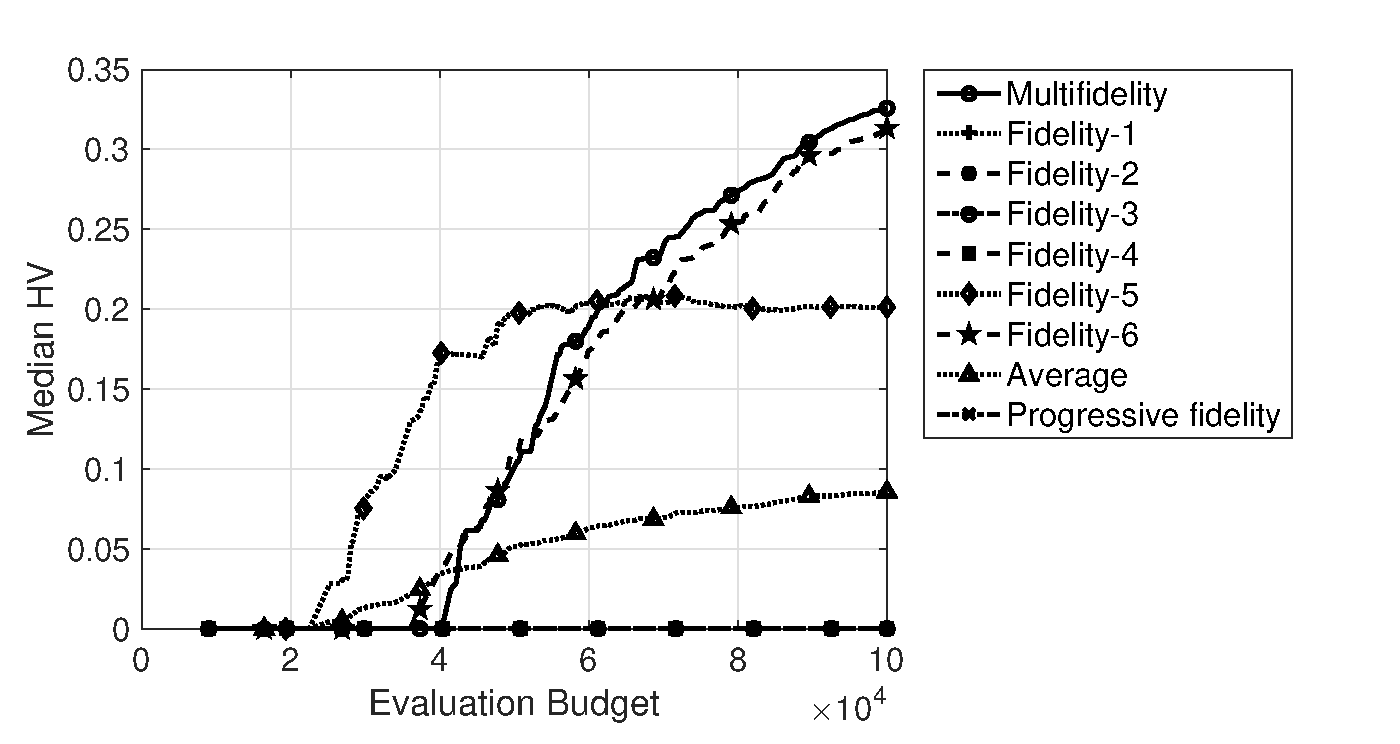
\includegraphics[scale=.35]{Figures/test_new_g_HV.eps}
	\caption{Test function-IV: Convergence at $s_{th}$ = 1}
	\label{fig:Meanplot_test_new_g_1sigma}
\end{figure}

Final statistics for all runs corresponding to various approaches are listed in Table \ref{tab:testfunc4hvstat}. Once again the superior performance of PD-MFEA is evident. 

\begin{table}[!htb]\footnotesize
	\centering
	\caption{Test function-IV: Final HV values of multi-fidelity, single fidelity optimization and progressive fidelity optimization}
	\label{tab:testfunc4hvstat}
	\begin{tabular}{|c|c|c|c|c|c|}
		\noalign{\smallskip}\hline
		Solver& Best &Mean & Median & Worst & Std Error\\ \hline
		$MF$&0.389&0.304&\textbf{0.326}&0.000&0.008\\ \hline
		$SF^1$&0.000&0.000&0.000&0.000&0.000\\ \hline
		$SF^2$&0.000&0.000&0.000&0.000&0.000\\ \hline
		$SF^3$&0.000&0.000&0.000&0.000&0.000\\ \hline
		$SF^4$&0.000&0.000&0.000&0.000&0.000\\ \hline
		$SF^5$&0.246&0.202&0.201&0.137&0.002\\ \hline
		$SF^6$&0.374&0.283&0.313&0.000&0.008\\ \hline
		$PF$&0.200&0.009&0.000&0.000&0.003\\ 
		\hline
	\end{tabular}
\end{table}

\subsection{Performance Score}

Based on the median values of objective (for single objective optimization problems) and HV (for multi-objective optimization problems) at the end of computational budget, we further compute the performance score \cite{bader2011hype} to quantify the overall performance of multi-fidelity, lowest fidelity, highest fidelity and progressive fidelity approaches. 

For a problem instance, suppose there are $n$ approaches ($SV_1$, $SV_2$, $\ldots$, $SV_n$). If the performance of the $i^{th}$ approach ($SV_i$) is significantly better (using Kolmogorov-Smirnov test at $5\%$ significance level) than the $j^{th}$ approach ($SV_j$) in terms of either median HV or objective value at the end of the evaluation budget, $\delta_{i,j}$ is considered to be $1$ and $0$ otherwise. Thus, for the $i^{th}$ approach ($SV_i$), it's performance score $P(SV_i)$ is determined as:\\

$P(SV_i)$ = $\sum_{j = 1,j\neq i}^n \delta_{i,j}$.\\

This performance score is averaged across all problems to compute the overall performance score of the approach. Therefore, a higher performance score is preferred. Figure \ref{fig:score} summarizes the overall performance score for the indicated approaches. It is clear that PD-MFEA (multi-fidelity approach) performs significantly better than the other approaches (lowest fidelity, highest fidelity and progressive fidelity approaches).

\begin{figure}[ht]
	\centering
	\includegraphics[scale=.35]{Figures/score.eps}
	\caption{Significance test}
	\label{fig:score}
\end{figure}

\section{Conclusion and Future Directions}
In this paper, we have introduced a novel approach for multi-fidelity optimization involving iterative solvers. The approach relies on a $(\mu+\lambda)$ evolutionary model, where solutions are only evaluated in higher levels of fidelity if they cannot be safely discarded as members of the parent population of the next generation. The predicted performance of a solution and its associated error in the highest fidelity is estimated based on its performance in its current fidelity level and information acquired from its neighboring solutions. This is subsequently used to compute the probabilistic dominance score of a solution amongst $(\mu+\lambda)$ solutions. This score, standard error associated with this score and the standard error threshold ($s_{th}$) is used to decide one of the following actions i.e., (a) discard (b) evaluate it in the next higher fidelity level or (c) preserve. The performance of the proposed approach has been illustrated using a number of unconstrained and constrained single and multi-objective optimization problems including two practical examples involving models constructed from partially convergence CFD simulations (a) design of an underwater vehicle for minimum drag and (b) identification of optimum flapping wing kinematics. The effect of standard error threshold and presence of redundant fidelity levels have also been studied to provide greater insights into the working of the approach. In its current form, the algorithm can deal with individual objectives defined using different levels of fidelity at different costs that is often required for solution of complex multidisciplinary design optimization problems. 

A number of possible extensions can follow and some of them are being pursued by the authors. The first aspect is to extend the prediction model to incorporate all information of neighboring solutions through local CoKriging models. While such an attempt is likely to involve more computational overhead, it certainly offers an opportunity to enrich the underlying approximation models which in turn could offer significant benefits in terms of rate of convergence. The second aspect would be to develop the approach further to deal with problems involving different variable types i.e. both ordinal and categorical. that are increasingly being encountered in design of novel materials.  

\section*{Appendix: Test function formulations}

\subsection{Test function-I}
{\small
	\begin{align}
		\begin{split} 
			SF^1 ={} &\{(x - 2)^2 + 1.2(x + 2)^2 + 2 + \frac{20}{1 + (x + 2)^2}\}r_1,\\
			SF^2 ={} &\{0.8(x - 2)^2 + 10\sin(\frac{\pi}{2}(x + 1)) + 1.8(x + 2)^2 + \frac{6}{5} + \\
			& \frac{20}{1 + (x + 2)^2}\}r_2,\\ 
			SF^3 ={} &\{0.3(x - 2)^2 + 10\sin(\frac{\pi}{2}(x + 1)) + 8\sin(\pi(x + \frac{3}{2})) \\ 
			& + 2(x + 2)^2 + \frac{2}{5} + \frac{40}{1 + (x + 2)^2}\}r_3,\\ 
			SF^4 ={} &\{10\sin(\frac{\pi}{2}(x + 1)) + 8\sin(\pi(x + \frac{3}{2})) + \\ 
			& 6\sin(2\pi(x + \frac{7}{4})) + 2.5(x + 2)^2 - \\ 
			& \frac{2}{5} + \frac{40}{1 + (x + 2)^2}\}r_4,\\ 
			SF^5 ={} &\{10\sin(\frac{\pi}{2}(x + 1)) + 8\sin(\pi(x + \frac{3}{2})) \\
			& + 6\sin(2\pi(x + \frac{7}{4})) + 4\sin(4\pi(x + \frac{15}{8})) \\ 
			& + 1.8(x + 2)^2 - \frac{6}{5}\}r_5,\\
			SF^6 ={} &\{10\sin(\frac{\pi}{2}(x + 1)) + 8\sin(\pi(x + \frac{3}{2})) \\
			& + 6\sin(2\pi(x + \frac{7}{4})) + 4\sin(4\pi(x + \frac{15}{8}))\\ 
			& + 2\sin(8\pi(x + \frac{31}{16})) + 2(x + 2)^2 - 2\}r_6,\\ \\
			&\text{where}~x~\in~[-10,6.5], r_i~(i = 1,\ldots,6) = 1
			\label{eq:testfunc1}
		\end{split}
\end{align}}%

\subsection{Test function-II}
{\small
	\begin{align*}
		\begin{split} 
			{SF_1}^1 ={} &\{40+(x_1 - 2)^2 + 1.2(x_1 + 2)^2 + 2 + \\ 
			&\frac{20}{1 +(x_1 + 2)^2}\}r_1,\\ 
			{SF_1}^2 ={} &\{40+0.8(x_1 - 2)^2 + 10\sin(\frac{\pi}{2}(x_1 + 1)) +\\ 
			& 1.8(x_1 + 2)^2 + \frac{6}{5} + \frac{20}{1 + (x_1 + 2)^2}\}r_2,\\
			{SF_1}^3 ={} &\{40+0.3(x_1 - 2)^2 + 10\sin(\frac{\pi}{2}(x_1 + 1)) +\\ 
			& 8\sin(\pi(x_1 + \frac{3}{2})) + 2(x_1 + 2)^2 + \frac{2}{5} +\\ 
			&\frac{40}{1 + (x_1 + 2)^2}\}r_3,\\ 
			{SF_1}^4 ={} &\{40+10\sin(\frac{\pi}{2}(x_1 + 1)) + 8\sin(\pi(x_1 + \frac{3}{2})) +\\ 
			& 6\sin(2\pi(x_1 + \frac{7}{4})) + 2.1(x_1 + 2)^2 \\
			&- \frac{2}{5} + \frac{40}{1 + (x_1 + 2)^2}\}r_4,\\
			{SF_1}^5 ={} &\{40+10\sin(\frac{\pi}{2}(x_1 + 1)) + 8\sin(\pi(x_1 + \frac{3}{2})) +\\ 
			& 6\sin(2\pi(x_1 + \frac{7}{4})) + 4\sin(4\pi(x_1 + \frac{15}{8})) +\\ 
			&1.9(x_1 + 2)^2 - \frac{6}{5}\}r_5,\\
		\end{split}
	\end{align*}
	\begin{align}
		\begin{split}
			{SF_1}^6 ={} &\{40+10\sin(\frac{\pi}{2}(x_1 + 1)) + 8\sin(\pi(x_1 + \frac{3}{2})) +\\ 
			& 6\sin(2\pi(x_1 + \frac{7}{4})) + 4\sin(4\pi(x_1 + \frac{15}{8})) +\\ 
			&2\sin(8\pi(x_1 + \frac{31}{16})) + 2(x_1 + 2)^2 - 2\}r_6,\\\\
			& \text{where}\\\\
			r_1 ={} &1 + ackley(\{(x_2 - 0.60) (x_3 - 0.50)\}),\\
			r_2 ={} &1 + ackley(\{(x_2 - 0.50) (x_3 - 0.60)\}),\\
			r_3 ={} &1 + ackley(\{(x_2 - 0.40) (x_3 - 0.70)\}),\\
			r_4 ={} &1 + ackley(\{(x_2 - 0.30) (x_3 - 0.82)\}),\\
			r_5 ={} &1 + ackley(\{(x_2 - 0.24) (x_3 - 0.86)\}),\\ 
			r_6 ={} &1 + ackley(\{(x_2 - 0.20) (x_3 - 0.90)\}),\\ \\
			& \text{where}~x_1~\in~[-10,6.5], x_2, x_3~\in~[0,1],~\text{and} \\\\
			&ackley(\mathbf{x}) = -a~\exp\{-b\sqrt{\frac{1}{d}\sum_{i = 1}^d x^2_i}\} -\\ 
			& \exp\{\frac{1}{d}\sum_{i = 1}^d \cos(c~x_i)\} + a + \exp(1) \\
			& a = 20, b = 0.2, c = 2\pi,~\text{and}~d = 2\\
			& {SF_1}^i~\text{indicates}~i^{th}~\text{fidelity value in the first objective}
			\label{eq:testfunc2}
		\end{split}
\end{align}}%

\subsection{Test function-III}
{\small
	\begin{align}
		\begin{split} 
			SF^i ={} & A\exp^{-\zeta\omega{|x-3|}^i}\sin(\omega_dx+\phi) \\
			g^i = {} & A\exp^{-\zeta\omega{|x-3|}^i}\sin(\omega_dx+\phi) + 0.8 <= 0 \\\\
			&\text{where}\\ \\
			\omega ={} &\sqrt{\frac{k_i}{m}},~A = \sqrt{\frac{(\zeta\omega)^2 + \omega^2_d}{\omega^2_d}},\\
			\zeta ={} &\frac{c}{2m\omega},~\omega_d = \omega\sqrt{1-\zeta^2},\\
			\phi ={} &\tan^{-1}\frac{\omega_d}{\zeta\omega},\\
			m ={} & 0.7, c = 0.8, i \in (1,2,3,4,5), \\
			&k_i \in (12,12.5,12.7,12.8,13)~\text{for}~SFi,\\
			&k_i \in (12.75,13.5,14.3,15.1,16.9)~\text{for}~ci\\
			&g^i~\text{is constraint function value in}~i^{th}~\text{fidelity}
			\label{eq:testfunc3}
		\end{split}
\end{align}}%

\subsection{Test function-IV}
\noindent Objective formulation is same as Test function-III. For the constraint formulation, \\
{\small
	\begin{align}
		\begin{split}
			g^i = {}&-(1 - ({SF_2}^i - 40)/38 - ({SF_1}^i - 40)/37) <= 0\\
			&\text{where}~g^i~\text{is the constraint function value in}~i^{th}~\text{fidelity}\\
			\label{eq:testfunc4} 
		\end{split}
	\end{align}
}%
where ${SF_1}^i$ indicates $i^{th}$ fidelity value of the first objective and ${SF_2}^i$ indicates $i^{th}$ fidelity value of second objective.
 
